\documentclass{foi}
\usepackage[utf8]{inputenc}
\usepackage{lipsum}

\vrstaRada{\diplomski}
\title{Razvoj polustrukturirane baze podataka za potrebe internetskog foruma kao web-aplikacije}

\author{Dario Bogović}
\spolStudenta{\musko}
\mentor{Bogdan Okreša Đurić}
\spolMentora{\musko}
\godina{2020}
\mjesec{rujan}
\date{2020}
\indeks{47165}
\smjer{Informacijsko i programsko inženjerstvo}
\titulaProfesora{Dr. sc.}

\sazetak{Rad se sastoji od teorijskog i praktičnog dijela. U teorijskom dijelu opisan je polustrukturirani model podataka, definirane razlike u odnosu na strukturirane i nestrukturirane podatke te predstavljeni tipovi polustrukturiranih podataka, s naglaskom na XML. Slijedi opis i definiranje XML baze podataka te pregled sustava za upravljanje XML bazom podataka. Praktični dio rada sadrži prikaz rada s noSQL dokumentnom bazom podataka i programskom platformom eXist-db, uz izradu konkretne XML baze podataka. Načini pristupa XML bazi podataka, slanje upita i dohvaćanje podataka prikazani su na primjeru Java web-aplikacije za internetski forum.}

\kljucneRijeci{xml; polustrukturirani podaci; XML baza podataka; eXist-db}

\begin{document}

\maketitle

\tableofcontents

\pagestyle{plain}
\chapter{Uvod}

Obavezno napiši zašto? Zašto je ovo dobro koristiti? Zašto baš s time itd.?

Završni ili diplomski rad studenta/studentice je konačni rezultat uloženog napora u završetak studija. Obranom završnog ili diplomskog rada student/studentica stječe prava i obveze koje proizlaze iz završetka akademskog obrazovanja. S ciljem osiguranja potpore studentima pri pisanju završnog/diplomskog rada, izrađen je ovaj predložak oblikovanja samog rada.

Načelna napomena o strukturi rada jest da se nazivi i struktura poglavlja obavezno definiraju u dogovoru s mentorom/mentoricom. Sadržajna preporuka je da u uvodu treba opisati što je tema završnog/diplomskog rada, zašto je tema značajna te koja je motivacija studenta/ studentice za odabir teme. 

\chapter{Podaci}

\lipsum[1]

\section{Strukturirani podaci}

\lipsum[1]

\section{Nestrukturirani podaci}

\lipsum[1]

\section{Polustruktirani podaci}

\lipsum[1]

\chapter{XML}

\lipsum[1-2]

\chapter{XML baza podataka}

\lipsum[1]

\section{eXist-db}

\lipsum[1]

\chapter{Opis aplikacijske domene}

Kao praktični dio ovog rada izradit će se XML baza podataka na programskoj platformi eXist-db za potrebe internetskog foruma. Aplikacija koja će koristiti izrađenu bazu podataka će biti realizirana kao Java web-aplikacija. U ovom poglavlju će se definirati internetski forum koji je aplikacijska domena praktičnog dijela rada. Zatim slijedi opis funkcionalnosti izrađene web-aplikacije pod nazivom "Diskuto".

\section{Internetski forum}

Internetski forum je web-aplikacija koja pruža komunikaciju između više ljudi o nekoj određenoj temi. Sudionici na forumu su najčešće anonimni, a eventualno za sudjelovanje u njemu se može zahtijevati registracija sa korisničkim imenom i lozinkom.  Sve poruke koje korisnik napiše i pošalje su vidljive svim ostalim sudionicima. \cite{definitionInternetForum} Zbog toga se internetski forum ponekad naziva oglasna ploča (eng. discussion board). Poruke se mogu ostavljati i čitati bez ograničenja. Radi lakšeg snalaženja forum je podijeljen u nekoliko kategorija prema temama razgovora. Unutar njih se nalaze objave koje otvaraju i započinju korisnici. Postoji više vrsta korisnika:

\begin{itemize}
\item Neregistrirani korisnici, zovu se još i gosti, nemaju pravo sudjelovati u raspravama, ali zato mogu čitati i pregledavati sadržaj. Poneki forumi striktno zahtijevaju registraciju korisnika kako bi mogao i čitati forum. Postoje korisnici koji su vrlo česti posjetioci foruma, ali ne sudjeluju u njemu već samo pregledavaju objave. U Internet slangu takav korisnik se naziva "lurker".\cite{lurker}
\item Registrirani korisnici su obični korisnici koji sudjeluju u raspravama, otvaraju objave, komentiraju i tako pridonose internetskom forumu.
\item Moderatori (kratica "mod") su registrirani korisnici koji imaju prava poput: brisanja, spajanja, premještanja, razdvajanja, zaključavanja ili uređivanja objava. Mogu blokirati, odblokirati, suspendirati ili upozoravati obične korisnike foruma, sve u svrhu boljeg održavanja foruma.
\item Administratori (kratica "admin") su registrirani korisnici koji vode internetski forum. Mogu promovirati korisnike na moderatore, upravljati pravilima, kreirati sekcije, te raditi operacije nad bazom podataka. Administratori imaju ovlasti, ali i često rade kao moderatori.\cite{adminvsmoderator}
\end{itemize}

Osim gore opisanog, postoje još neke funkcionalnosti koje su sadržane na većini internetskih foruma. Privatne poruke (kratica "PM") služe za slanje privatne poruke od jednog korisnika prema drugom korisniku. Obično se takve poruke koriste za osobnu komunikaciju. Korisnik može prilikom slanja uz poruku učitati i datoteku kao prilog. Datoteka se pritom sprema na poslužitelj od foruma, stoga se moraju definirati ograničenja nad datotekama (tip datoteke i veličina datoteke). Osim u tekstualnom formatu, korisnik može objaviti poruku koristeći HTML. Kroz internetske forume su popularizirani i emotikoni ili smajlići, odnosno slikovni prikaz korisnikovog raspoloženja ili osjećanja. Korisnik može drugog korisnika staviti na listu ignoriranja čime neće više vidjeti njegove objave. Mnogi forumi omogućuju korisnicima da postave svoj potpis (kratica "sig") koji postaje vidljiv na kraju svake korisnikove objave. Korisnik se može i pretplatiti na pojedine dijelove foruma, da ne bi propustio sadržaj objavljen sa tog dijela foruma.\cite{vbulletinhelp}

Svaki forum sadrži i popis pravila kojih se korisnici moraju pridržavati. Kršenje pravila sankcioniraju administratori i moderatori, a nepridržavanje pravila mogu prijaviti i obični korisnici. Ako netko prekrši pravilo foruma, prvo ga se obično upozori preko privatne poruke. Ako korisnik nastavlja kršiti pravila zabranjuje mu se pristup forumu na određeni broj dana. Ako i dalje nastavlja kršiti pravila produžuje mu se zabrana pristupa forumu, a može dobiti i trajnu zabranu. Sadržaj koji krši pravila se obično obriše, a ponekad i tema koja je kontroverzna se zaključa i onemogući se korisnicima daljnja rasprava. \cite{rules}

Internetski forumi postoje još od samih početaka Interneta. Prve online zajednice i forumi su bili razvijani na BBS (eng. Bulletin Board System) 70-tih godina prošlog stoljeća. Najraniji takvi forumi su bili EIES (nastao 1976. godine) i KOM (nastao 1977. godine). The WELL je najstariji aktivni forum. Razvijen je 1985. godine, ali nije pretjerano popularan jer ima oko 2700 članova. \cite{forumhistory} Neki najpopularniji svjetski forumi su: 4chan, Bodybuilding.com, Stack Overflow, XDA-Developers, Quora i Reddit. U Hrvatskoj su najpoznatiji forum.bug.hr, indexforum, satelitski forum, teen385. Najstariji i najpoznatiji je Forum.hr. Razvijen je 1999. godine i sadrži preko 500.000 korisnika.

\begin{figure}[h!]
    \centering
    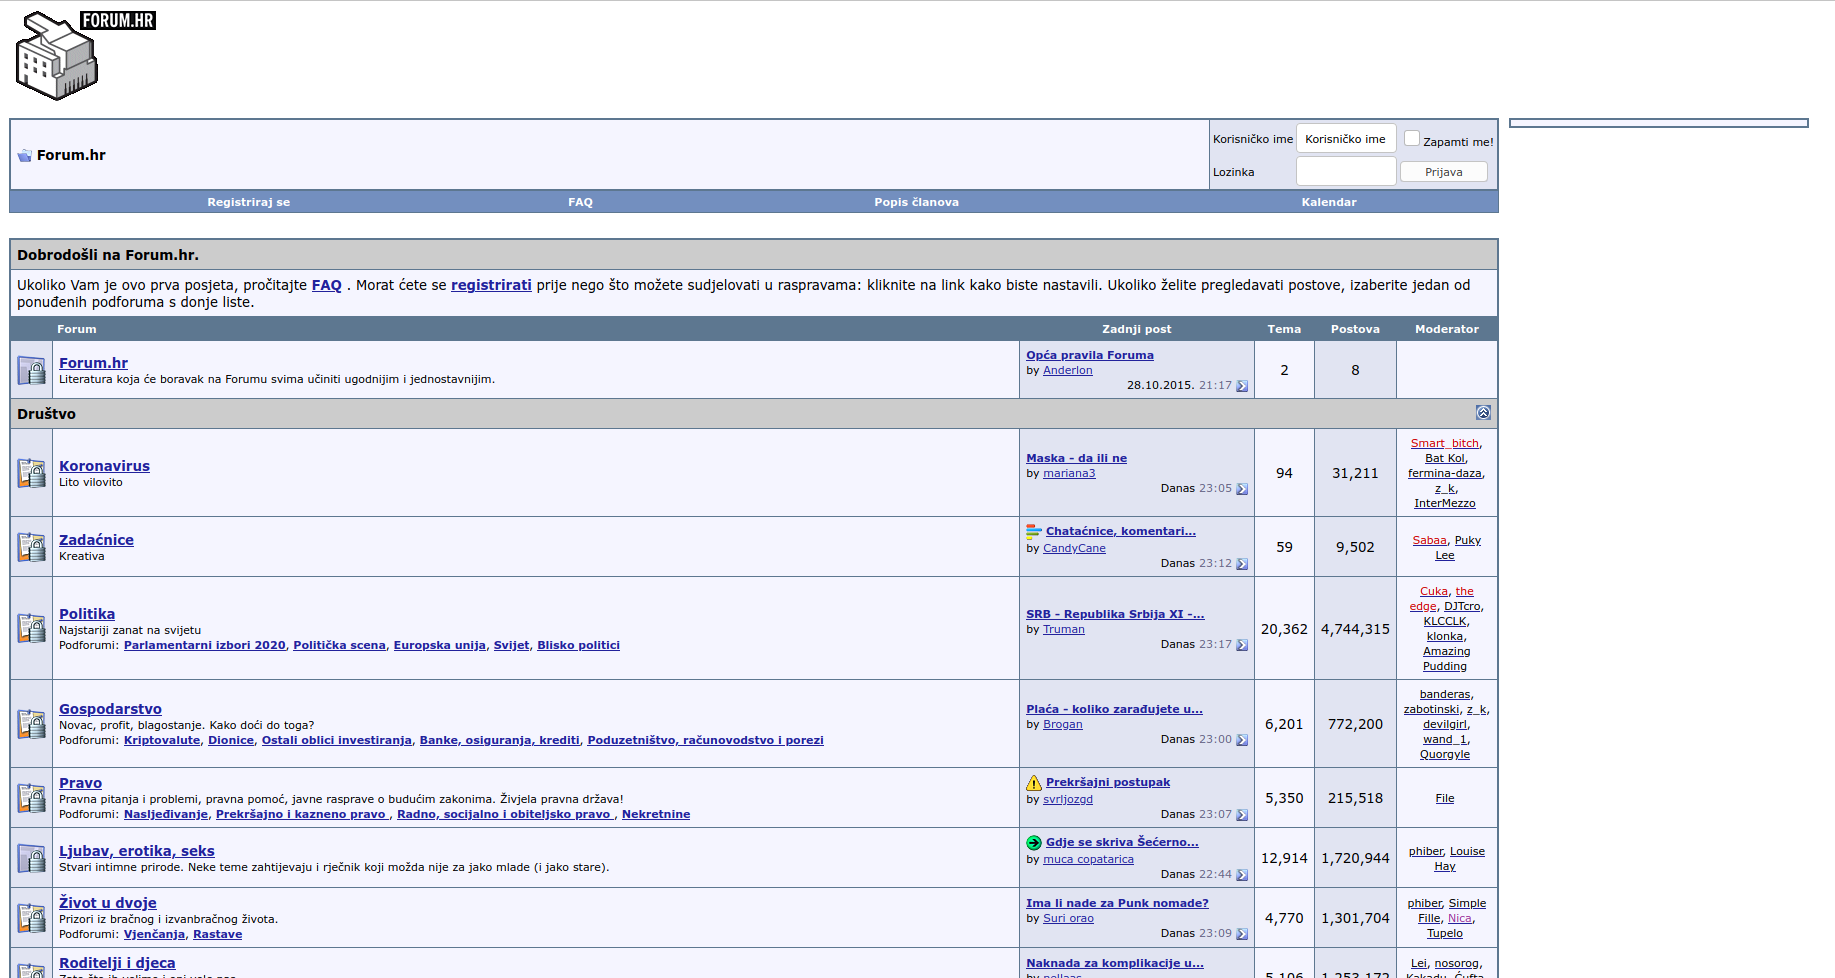
\includegraphics[width=1\textwidth]{slike/forumhr.png}
    \caption{Slika zaslona foruma Forum.hr}
\end{figure}

\section{Diskuto}

Diskuto je naziv internetskog foruma koji je razvijen kao praktični dio ovog rada. Naziv "Diskuto" dolazi od esperanto riječi koja u prijevodu znači "rasprava". Aplikacija objedinjuje funkcionalnosti najpoznatijeg svjetskog i najpoznatijeg domaćeg internetskog foruma: Reddit i Forum.hr.

Diskuto je aplikacija koja pruža korisnicima raspravu o nekoj određenoj temi. Aplikacija se sastoji od više različitih foruma (Diskuta) u kojima korisnici mogu pokretati različite objave i raspravljati o njima. Forum predstavlja lokaciju na kojoj korisnici pokreću objave sukladno pravilima svakog pojedinog foruma. Kako bi bio pregledniji, svaki forum se može dodatno razgranati po pojedinim kategorijama. Korisnici kada žele otvoriti novu objavu moraju joj zadati naslov, opis (tekstualni ili slikovni) i definirati na kojem forumu i u kojoj kategoriji tog foruma žele otvoriti objavu. Drugi korisnici se zatim mogu javljati, komentirati objavu i tako sudjelovati u raspravi o nekoj temi. Ako neka objava ili komentar krši pravila foruma, moderator može reagirati i obrisati ili zaključati objavu ili komentar. Svaki korisnik može svaku objavu i komentar označiti sa "+" ako ju smatra korisnom i zanimljivom ili sa "-" ako ju smatra lošom i krivom. Nad svakom takvom objavom se računa "karma", odnosno omjer pluseva i minusa. Na taj način može se lako vidjeti koje su objave i komentari kvalitetni, a koji to nisu. Karma se preslikava i na korisnika koji je kreirao objavu ili komentar, te je vidljiva javno na njegovom profilu. Tako se može vidjeti koliko korisnik doprinosi svojim sudjelovanjem. Na Diskutu postoje sljedeće vrste korisnika:

\begin{itemize}
\item Neregistrirani korisnik - nema pravo sudjelovati u raspravama, ali zato može čitati i pregledavati sadržaj. Može otvarati forume (Diskuta), pregledavati kategorije i pregledavati raspravu na pojedinim objavama.
\item Registrirani korisnik - može čitati forume, pregledavati kategorije i pregledavati raspravu na pojedinim objavama, kreirati svoje forume, pretplatiti se na tuđe forume, kreirati nove objave na svojim ili tuđim forumima, sudjelovati u raspravama na svojim ili tuđim objavama, brisati svoje objave ili komentare, prijavljivati tuđe objave ili komentare moderatorima pojedinog foruma, dati "+" ili "-" objavi ili komentaru, pregledavati tuđe profile, slati i primati privatne poruke od drugih korisnika, uređivati svoj korisnički profil, mijenjati jezik aplikacije, pretraživati forume, objave ili profile.
\item Vlasnik - registrirani korisnik koji kada kreira svoj forum, on postaje vlasnik na tom forumu. Ima pune ovlasti nad forumom što uključuje: uređivanje opisa i pravila, dodavanje i brisanje kategorija, davanje ili oduzimanje moderatorskih ovlasti drugim korisnicima, pregled prijavljenih objava i komentara na svom forumu, brisanje tuđih objava i komentara sa svog foruma, zaključavanje pojedinih objava.
\item Moderator - registrirani korisnik koji nije kreirao forum, ali su mu dodijeljene sve ovlasti nad forumom koje ima i vlasnik. Razlika u odnosu na vlasnika je i to što vlasnik ima trajne i neopozive ovlasti nad forumom, dok se moderatoru u svakom trenutku može uskratit ovlasti čime na tom forumu onda postaje obični registrirani korisnik.
\end{itemize}

\begin{figure}[h!]
    \centering
    
\includegraphics[width=0.5\textwidth]{slike/logo.png}
    \caption{Logo aplikacije Diskuto}
\end{figure}

Registracija se obavlja na način da korisnik unosi željeno korisničko ime i lozinku, te e-mail na koji će mu stići kod sa kojim će potvrditi registraciju. U aplikaciju se prijavljuje koristeći se korisničkim imenom i lozinkom, a ako je zaboravio lozinku može ju i poništiti. Osim javnog raspravljanja na objavama, korisnici si mogu i međusobno razmijenjivati privatne poruke. Diskuto je dostupan na dva jezika: engleskom i hrvatskom. Promjena jezika se izvršava u postavkama, gdje si korisnik može urediti svoje korisničke podatke ili obrisati svoj račun.

\chapter{Model baze podataka}

Baza podataka se sastoji od kolekcije u kojoj se nalazi 4 XML dokumenta: forumi (forums.xml), poruke (messages.xml), objave (posts .xml) i korisnici (users.xml). To su ujedno i osnovni koncepti prepoznati iz aplikacijske domene. U nastavku je prikazana XML schema svih XML dokumenata u kolekciji "db/diskuto", te njihov opis.

\section{Korisnici (users.xml)}

XML dokument "users.xml" sadrži popis svih korisnika u aplikaciji. Registracijom se dodaje novi korisnik (<user/>). Elemente "email" (elektronička pošta korisnika), "name" (korisničko ime) i "password" (lozinka) definira korisnik prilikom registracije. Prilikom registracije aplikacija u pozadini dodijeljuje element "created" koji predstavlja UNIX vrijeme u koje je korisnik kreirao račun i element "code" koji predstavlja kod za potvrdu registracije. Element "subscriptions" sadrži popis svih foruma na koje se korisnik pretplatio, a element "ignore" listu svih korisnika koje je ignorirao. Element "disabled" može poprimiti vrijednosti 0 ili 1, a on označava je li korisnik obrisao svoj račun. Element "language" može poprimiti vrijednosti 'en' i 'hr', a on označava jezik na kojem se aplikacija izvršava za tog korisnika.

\begin{lstlisting}[language=XML]
 <?xml version="1.0"?>
<xs:schema xmlns:xs="http://www.w3.org/2001/XMLSchema">

<xs:element name="users">
   <xs:complexType>
      <xs:element name="user">
         <xs:complexType>
            <xs:sequence>
              <xs:element name="email" type="xs:string"/>
              <xs:element name="name" type="xs:string"/>
	      <xs:element name="password" type="xs:string"/>
	      <xs:element name="code" type="xs:integer"/>
	      <xs:element name="created" type="xs:integer"/>
	      <xs:element name="subscriptions">
	         <xs:complexType>
	           <xs:sequence>
		      <xs:element name="forum" type="xs:string"/>
		   </xs:sequence>
	         </xs:complexType>
	      </xs:element>
	      <xs:element name="ignore">
                <xs:complexType>
	           <xs:sequence>
		      <xs:element name="user" type="xs:string"/>
 		   </xs:sequence>
		</xs:complexType>
	      </xs:element>
	      <xs:element name="disabled" type="xs:boolean"/>
	      <xs:element name="language" type="languageType"/>
	      <xs:simpleType name="languageType">
	         <xs:restriction base="xs:string">
		   <xs:enumeration value="en"/>
		   <xs:enumeration value="hr"/>
	         </xs:restriction>
	      </xs:simpleType>
	    </xs:sequence>
	 </xs:complexType>
      </xs:element>
   </xs:complexType>
</xs:element>

</xs:schema> 
\end{lstlisting}

\section{Forumi (forums.xml)}

XML dokument "forums.xml" sadrži popis svih foruma u aplikaciji. Nakon što korisnik kreira u aplikaciji novi forum, podaci o njemu se spremaju u ovom dokumentu. Prilikom kreiranja foruma postavljaju se elementi: "name" (naziv foruma), "description" (opis foruma), "categories" (sadrži popis svih kategorija), "moderators" (popis svih moderatora) i "rules " (pravila foruma). Nad forumom postoje još elementi "owner" (označava korisnika koji je vlasnik foruma), "created" (UNIX vrijeme u koje je forum kreiran) i "subscribers" (broj pretplaćenih korisnika na forumu).

\begin{lstlisting}[language=XML]
 <?xml version="1.0"?>
<xs:schema xmlns:xs="http://www.w3.org/2001/XMLSchema">

<xs:element name="forums">
   <xs:complexType>
      <xs:element name="forum">
         <xs:complexType>
            <xs:sequence>
              <xs:element name="name" type="xs:string"/>
              <xs:element name="description" type="xs:string"/>
	      <xs:element name="categories">
	         <xs:complexType>
	           <xs:sequence>
		      <xs:element name="category" type="xs:string"/>
		   </xs:sequence>
	         </xs:complexType>
	      </xs:element>
              <xs:element name="owner" type="xs:string"/>
	      <xs:element name="moderators">
	         <xs:complexType>
	           <xs:sequence>
		      <xs:element name="moderator" type="xs:string"/>
		   </xs:sequence>
	         </xs:complexType>
	      </xs:element>
              <xs:element name="rules" type="xs:string"/>
	      <xs:element name="created" type="xs:integer"/>
	      <xs:element name="subscribers" type="xs:integer"/>
            </xs:sequence>
         </xs:complexType>
      </xs:element>
   </xs:complexType>
</xs:element>

</xs:schema> 
\end{lstlisting}

\section{Objave (posts.xml)}

XML dokument "posts.xml" sadrži popis svih objava na svim forumima u aplikaciji. Prilikom kreiranja objave, u ovom dokumentu se spremaju sve informacije o njoj.  Elementi koje sadrži svaka objava su: "id" (jedinstveni identifikator objave), "headline" (naslov objave), "description" (tekstualni opis objave), "attachment" (slikovni opis objave), "created" (UNIX vrijeme u koje je objava kreirana), "owner" (korisnik koji je kreirao objavu), "diskuto" (forum na kojem je objavljena), "category" (kategorija na forumu na kojem je objavljena), "upvote" (svi korisnici koji su označili objavu sa '+'), "downvote" (svi korisnici koji su označili objavu sa '-'), "reported" (može poprimiti vrijednost 0 ili 1 i označava je li objava prijavljena moderatorima), "deleted" (može poprimiti vrijednost 0 ili 1 i označava je li objava obrisana), "locked" (može poprimiti vrijednost 0 ili 1 i označava je li objava zaključana), element "comments" koji predstavlja sve komentare koje sadrži pojedina objava. Svaki komentar ("comment") u sebi sadrži atribute: "id" (identifikator komentara na toj objavi), "text" (sami tekst objave), "created" (UNIX vrijeme u kojem je objava kreirana), "owner" (označava korisničko ime korisnika koji je vlasnik komentara), "upvote" (svi korisnici koji su označili komentar sa '+'), "downvote" (svi korisnici koji su označili komentar sa '-'), "reported" (može poprimiti vrijednosti 0 ili 1 i označava je li komentar prijavljen moderatorima) i "deleted" (može poprimiti vrijednosti 0 ili 1 i označava je li komentar obrisan).

\begin{lstlisting}[language=XML]
 <?xml version="1.0"?>
<xs:schema xmlns:xs="http://www.w3.org/2001/XMLSchema">

<xs:element name="posts">
   <xs:complexType>
      <xs:element name="post">
         <xs:complexType>
            <xs:sequence>
	      <xs:element name="id" type="xs:integer"/>
              <xs:element name="headline" type="xs:string"/>
              <xs:element name="description" type="xs:string"/>
              <xs:element name="attachment" type="xs:string"/>
	      <xs:element name="created" type="xs:integer"/>
              <xs:element name="owner" type="xs:string"/>
              <xs:element name="diskuto" type="xs:string"/>
              <xs:element name="category" type="xs:string"/>
	      <xs:element name="upvote">
	         <xs:complexType>
	           <xs:sequence>
		      <xs:element name="user" type="xs:string"/>
		   </xs:sequence>
	         </xs:complexType>
	      </xs:element>
	      <xs:element name="downvote">
	         <xs:complexType>
	           <xs:sequence>
		      <xs:element name="user" type="xs:string"/>
		   </xs:sequence>
	         </xs:complexType>
	      </xs:element>
	      <xs:element name="comments">
	         <xs:complexType>
	           <xs:sequence>
		      <xs:element name="comment">
		         <xs:complexType>
		            <xs:sequence>
		               <xs:element name="id" type="xs:integer"/>
		               <xs:element name="text" type="xs:string"/>
		               <xs:element name="created" type="xs:integer"/>
		               <xs:element name="owner" type="xs:string"/>
		               <xs:element name="upvote">
		                  <xs:complexType>
		                     <xs:sequence>
		                        <xs:element name="user" type="xs:string"/>
		                     </xs:sequence>
		                  </xs:complexType>
		               </xs:element>
		               <xs:element name="downvote">
		                  <xs:complexType>
		                     <xs:sequence>
		                        <xs:element name="user" type="xs:string"/>
		                     </xs:sequence>
		                  </xs:complexType>
		               </xs:element>
		               <xs:element name="reported" type="xs:boolean"/>
		               <xs:element name="deleted" type="xs:boolean"/>
		            </xs:sequence>
		         </xs:complexType>
		      </xs:element>
		   </xs:sequence>
	         </xs:complexType>
	      </xs:element>
	      <xs:element name="reported" type="xs:boolean"/>
	      <xs:element name="deleted" type="xs:boolean"/>
	      <xs:element name="locked" type="xs:boolean"/>
            </xs:sequence>
         </xs:complexType>
      </xs:element>
   </xs:complexType>
</xs:element>

</xs:schema> 
\end{lstlisting}

\section{Poruke (messages.xml)}

Sve poruke koje si korisnici međusobno šalju su sadržane u XML dokumentu "messages.xml". Kada korisnik pošalje privatnu poruku drugom korisniku, podaci se spremaju u ovom dokumentu. Elementi koji se zapisuju su: "sender" (korisničko ime korisnika koji je pošiljatelj poruke), "recipient" (korisničko ime korisnika koji je primatelj poruke), "time" (UNIX vrijeme u koje je poruka poslana), "text" (sadržaj poruke) i "seen" (može poprimiti vrijednosti 0 ili 1 i označava je li pošiljatelj vidio primljenu poruku).

\begin{lstlisting}[language=XML]
 <?xml version="1.0"?>
<xs:schema xmlns:xs="http://www.w3.org/2001/XMLSchema">

<xs:element name="messages">
   <xs:complexType>
      <xs:element name="message">
         <xs:complexType>
            <xs:sequence>
              <xs:element name="sender" type="xs:string"/>
              <xs:element name="recipient" type="xs:string"/>
              <xs:element name="time" type="xs:integer"/>
              <xs:element name="text" type="xs:string"/>
              <xs:element name="seen" type="xs:boolean"/>
            </xs:sequence>
         </xs:complexType>
      </xs:element>
   </xs:complexType>
</xs:element>

</xs:schema> 
\end{lstlisting}

\chapter{Implementacija}

\section{Kreiranje baze podataka}
\section{Rad s bazom podataka}
\section{Java web-aplikacija}

\chapter{Primjeri korištenja}

U ovom poglavlju ću opisati primjere korištenje izrađene web aplikacije. Svaka izrađena funkcionalnost će biti prikazana uz odgovarajuće slike zaslona i njihov opis.

\section{Početna stranica}

\begin{figure}[h!]
    \centering
    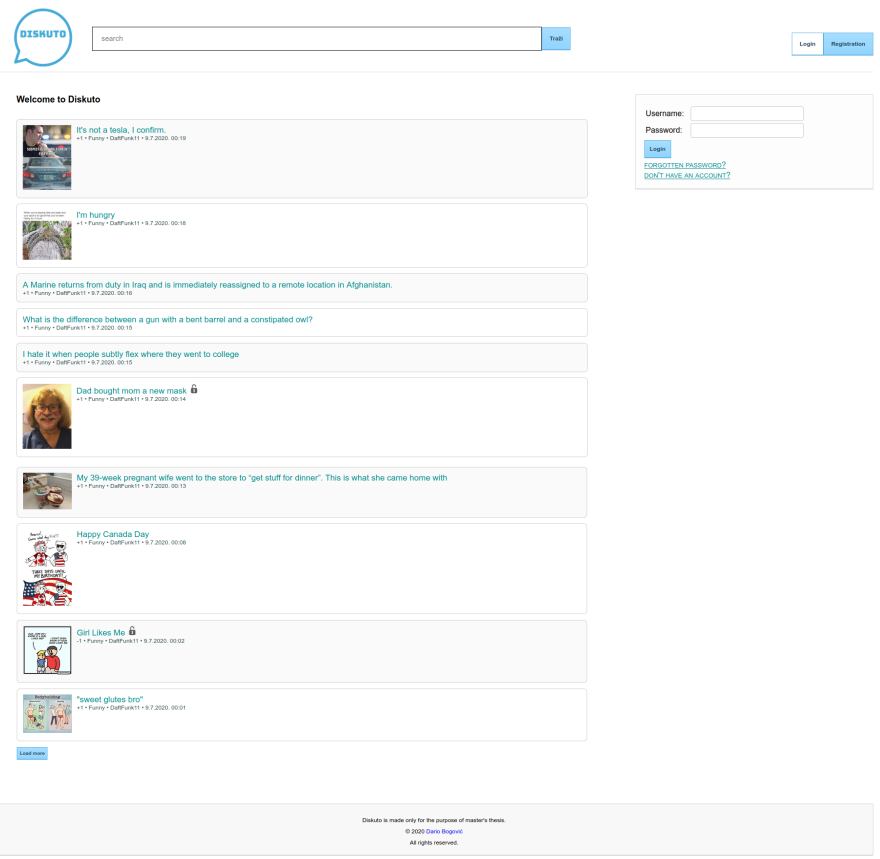
\includegraphics[width=1\textwidth]{slike/pocetna.png}
    \caption{Prikaz početne stranice (neprijavljen korisnik)}
    \label{pocetna}
\end{figure}

Na slici \ref{pocetna} je prikazana početna stranica web aplikacije. Sastoji se od tri dijela: zaglavlja stranice, podnožja stranice i glavnog dijela stranice. Zaglavlje stranice sadrži s lijeva na desno: logo, pretraživač web aplikacije i dvije poveznice koje vode na prijavu korisnika u aplikaciju ili na registraciju korisnika. Glavni dio početne stranice je prikazan u sredini i sadrži s desne strane blok element za brzu prijavu korisnika s poveznicama koje vode do forme za obnavljanje zaboravljene lozinke ili za registraciju novog korisnika. S lijeve strane glavnog dijela web aplikacije nalazi se poruka dobrodošlice i ispod koje poveznice na 10 najnovijih objava u aplikaciji. Na kraju se nalazi gumb za učitavanje dodatnih 10 objava. Podnožje stranice sadrži detalje o web aplikaciji i poveznicu na e-mail adresu autora.

\subsection{Početna stranica prijavljenog korisnika}

\begin{figure}[h!]
    \centering
    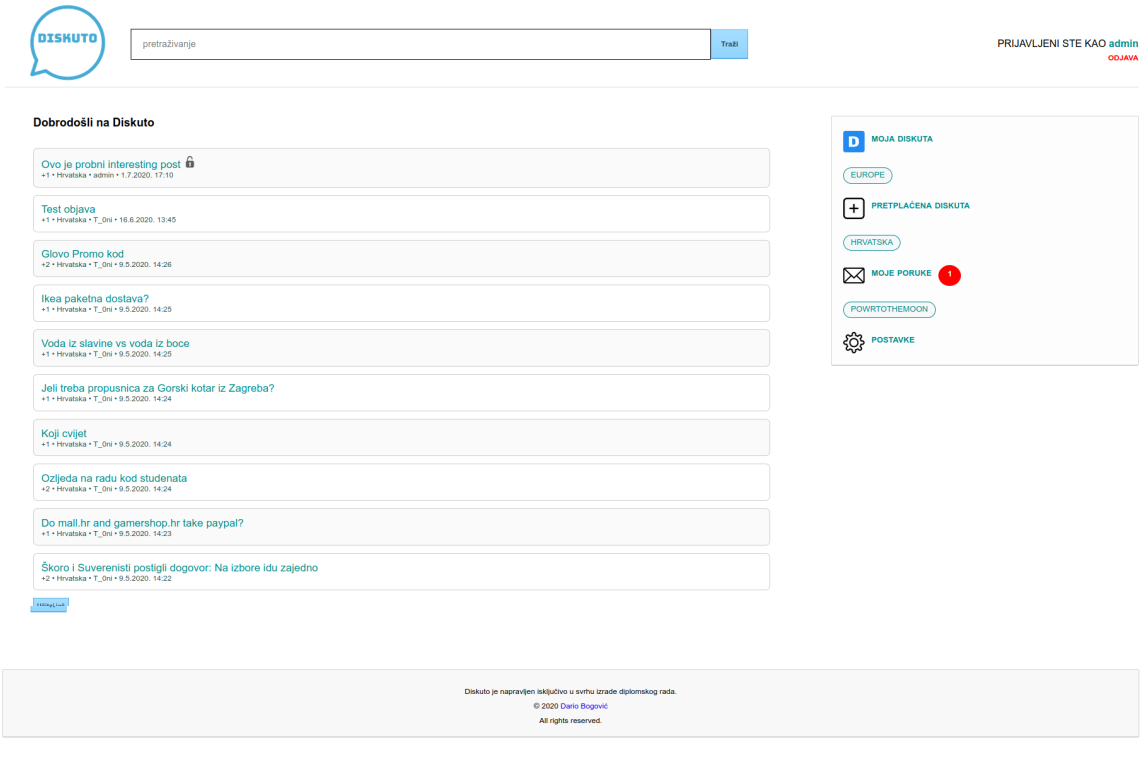
\includegraphics[width=1\textwidth]{slike/pocetna-prijavljen.png}
    \caption{Prikaz početne stranice (prijavljen korisnik)}
\end{figure}

Prijavom korisnika, bilo preko stranice namijenjene prijavi ili preko brze prijave, korisnika se preusmjerava na njegovu početnu stranicu. Za razliku od početne stranice neprijavljenog korisnika, kod prijavljenog korisnika ona sadrži u glavnom dijelu s lijeve strane popis najnovijih objava sa foruma na koje se korisnik pretplatio (za razliku od popisa najnovijih objava sa svih foruma), a sa desne strane glavni izbornik sa mogućnostima. U glavnom izborniku može se odabrati opcija "Moja Diskuta" koja korisnika vodi na stranicu sa svojim kreiranim forumima na kojem može kreirati forume ili im mijenjati postavke. Ispod poveznice na opciju se nalazi popis svih vlasititih foruma, te se klikom na njih može brzo pristupiti. Sljedeća mogućnost je "Pretplaćena Diskuta" koja korisnika vodi na stranicu za otkrivanje novih foruma na koje bi se korisnik mogao pretplatiti. Ispod poveznice se nalazi popis svih foruma na koje se korisnik pretplatio, te se njima može brzo pristupiti. Mogućnost "Moje poruke" korisnika vodi do stranice sa privatnim porukama. S desne strane se može vidjeti broj nepročitanih poruka koje korisnik ima, a ispod poveznice se može brzo pristupiti razgovoru s korisnicima s kojima ima nepročitanih poruka. Zadnja opcija u glavnom izborniku su "Postavke" koje korisnika vode do stranice sa postavkama korisničkog računa. U zaglavlju stranice, s desne strane, je prikazan naziv trenutačno prijavljenog korisnika. Pritiskom na naziv otvara se javni profil korisnika. Ispod naziva, nalazi se poveznica "Odjava" koja korisnika odjavljuje iz aplikacije.

\section{Registracija}

Na početnoj stranici kod neprijavljenog korisnika, klikom na poveznicu "Registration" u zaglavlju stranice ili "Don't have an account?" u glavnom dijelu stranice, otvara se web stranica sa formom za registraciju korisnika u aplikaciji prikazana na slici \ref{registracija}.

\begin{figure}[h!]
    \centering
    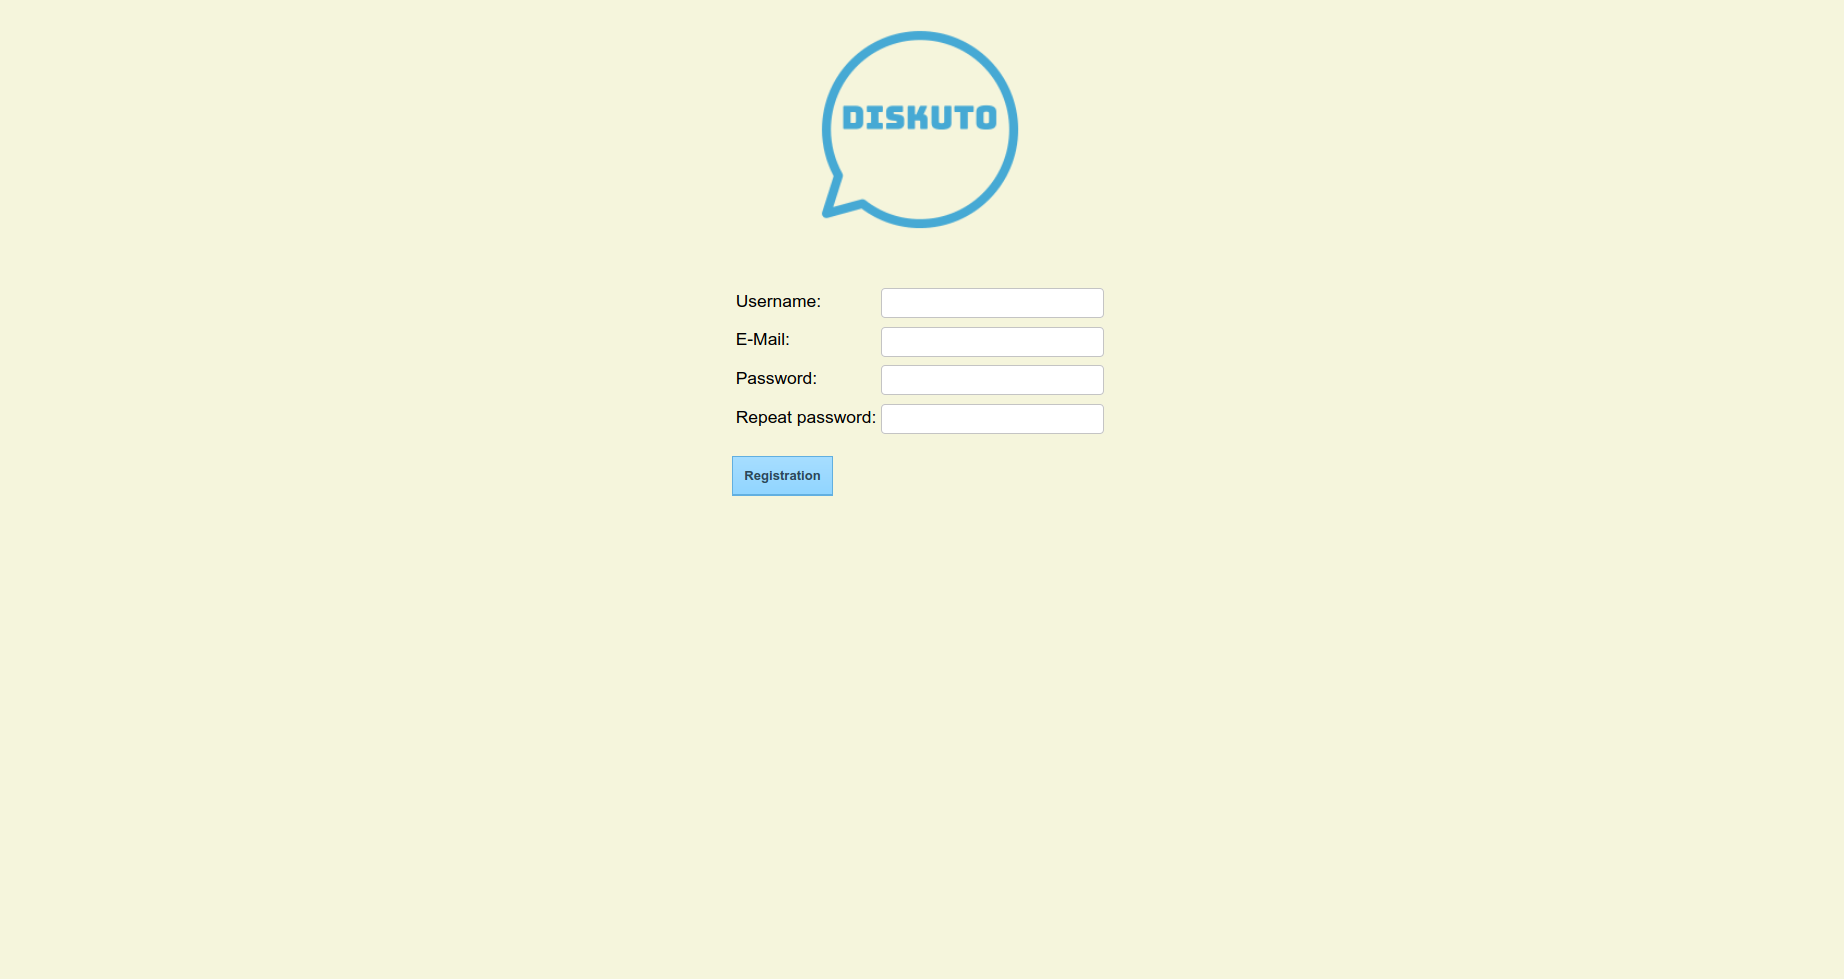
\includegraphics[width=1\textwidth]{slike/registracija.png}
    \caption{Forma za registraciju novog korisnika}
    \label{registracija}
\end{figure}

Prilikom registracije, korisnik mora unijeti željeno korisničko ime, e-mail, lozinku i ponoviti lozinku. Postoje nekoliko ograničenja prilikom registracije koja se moraju poštovati:

\begin{itemize}
\item Svi podaci moraju biti obavezno uneseni
\item Korisničko ime i e-mali ne smije postojati u bazi; svako korisničko ime se veže za isključivo jednog korisnika, te svaki e-mail se veže isljučivo za jednog korisnika
\item Korisničko ime ne smije biti kraće od 3 znaka, lozinka ne smije biti kraća od 8 znakova, a e-mail mora biti pravilnog formata
\item Unesena lozinka i ponovljena lozinka moraju biti jednake
\end{itemize}

Ukoliko neko ograničenje nije zadovoljeno, korisniku će se na zaslon ispisati poruka sa greškom. Tek kada je sve u redu sa unešenim podacima, u bazu se spremaju podaci i korisnika se preusmjerava na formu za potvrdu registracije. U međuvremenu, korisniku se dodijeljuju još neki meta-podaci: generira se kod za potvrdu koji će korisniku biti poslan na njegov e-mail, dodijeljuje mu se datum i vrijeme kada mu je kreiran račun, te se kao jezik aplikacije postavlja se engleski. Na kraju se šalje e-mail za potvrdu registracije.

\subsection{Potvrda registracije}

\begin{figure}[h!]
    \centering
    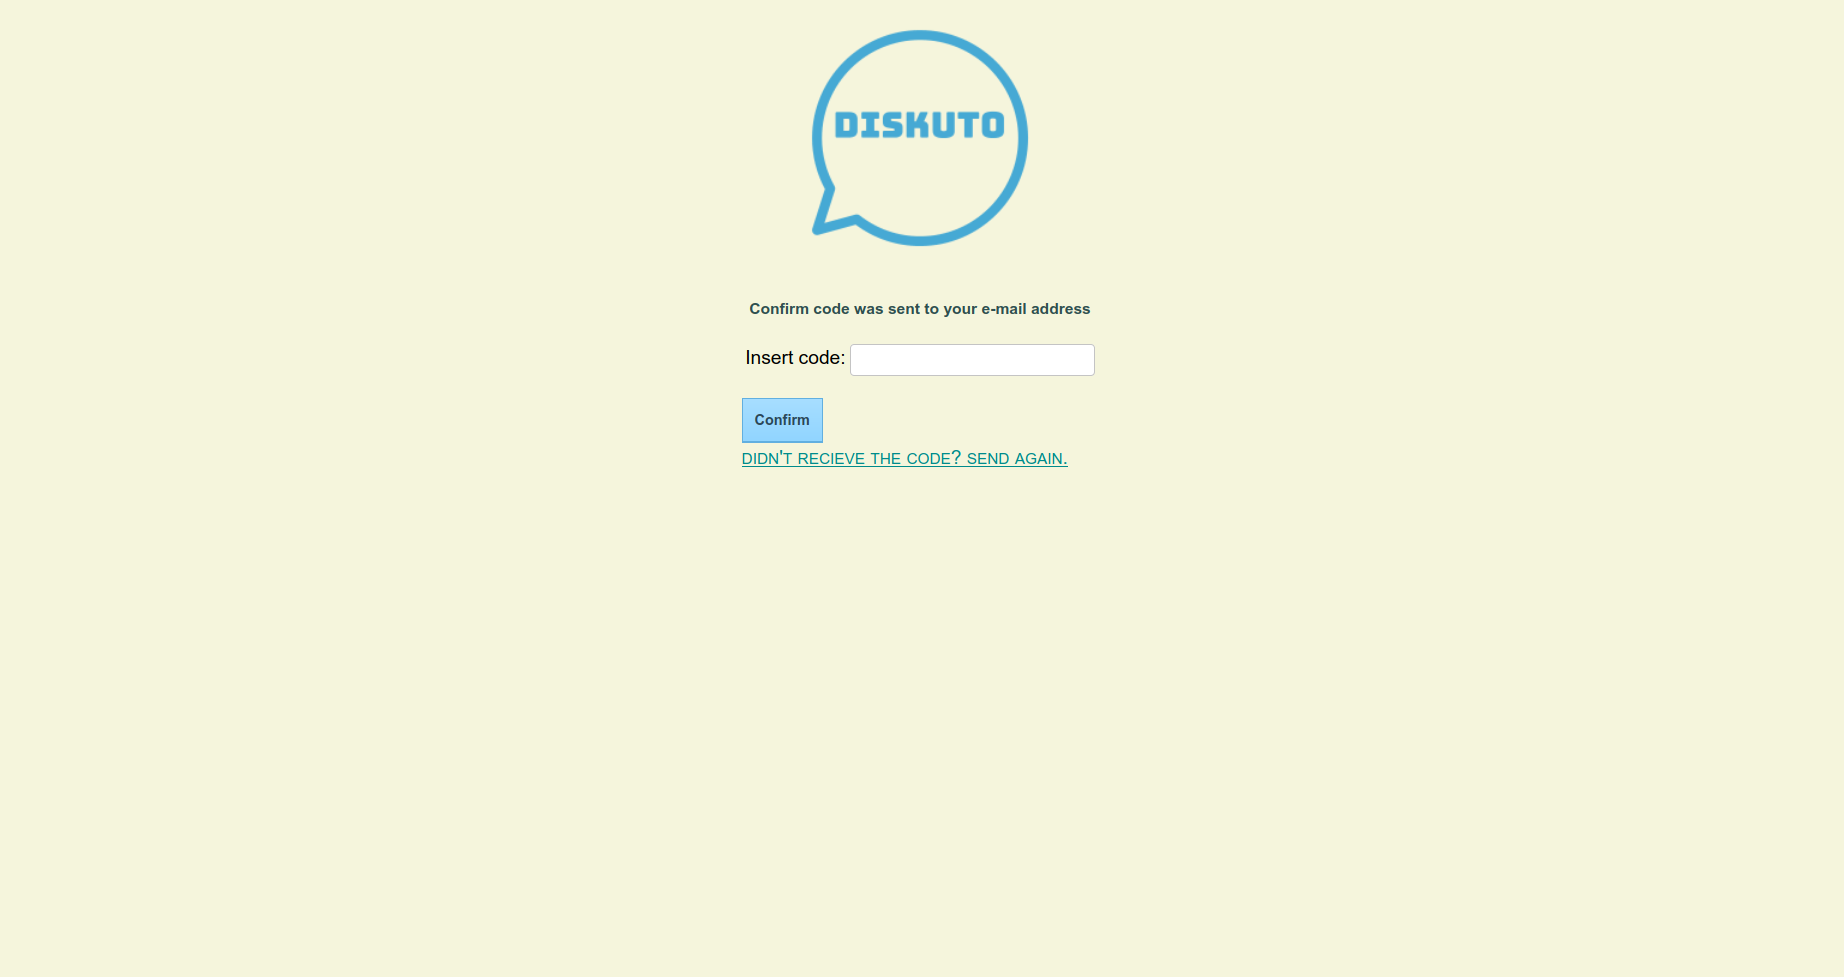
\includegraphics[width=1\textwidth]{slike/potvrda-registracije.png}
    \caption{Forma za potvrdu registracije novog korisnika}
    \label{potvrda-registracije}
\end{figure}

Na slici \ref{potvrda-registracije} je prikazana forma za potvrdu registracije novog korisnika. Kako bi potvrdio registraciju, korisnik mora unijeti šesteroznamenkasti kojeg je primio na mail. Ukoliko krivo unese kod, prikazuje mu se poruka greške. Ako je bilo problema oko primanja koda, korisnik može zatražiti ponovno slanje na njegov e-mail klikom na poveznicu "Send again". Tek kada unese ispravan kod, korisniku se potvrđuje registracija i postaje član Diskuta. Nepotvrđeni korisnici ne mogu se služiti aplikacijom, odnosno imaju iste ovlasti kao i drugi neregistrirani korisnici.

\begin{figure}[h!]
    \centering
    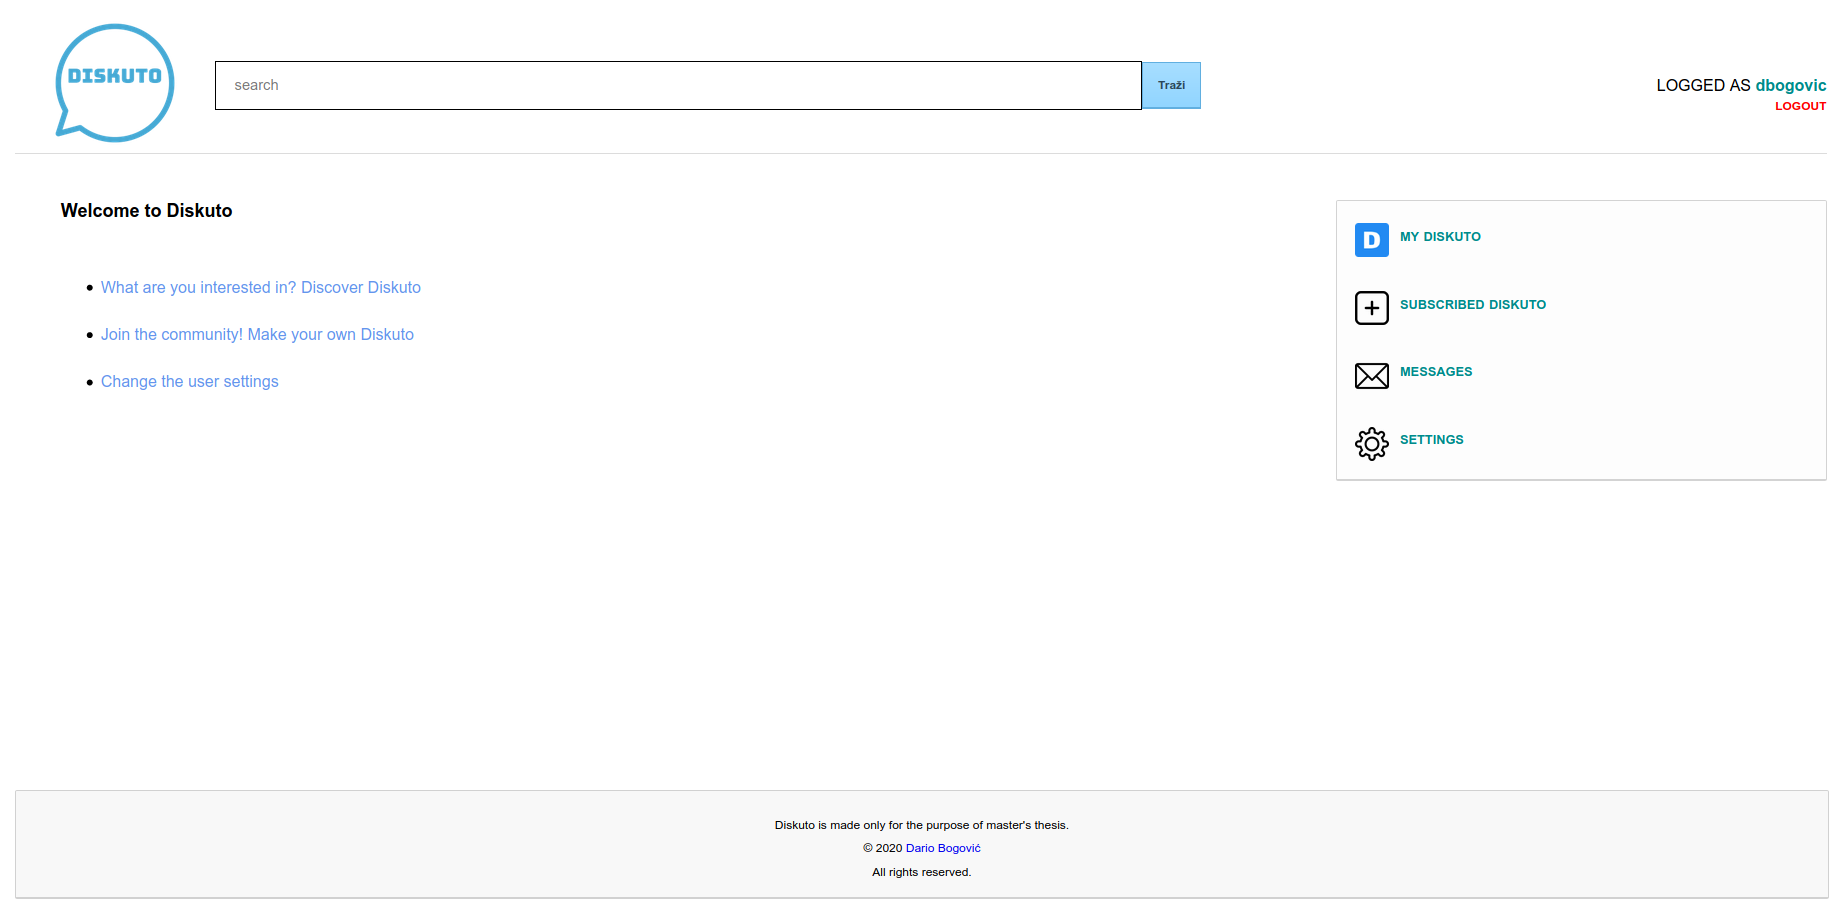
\includegraphics[width=1\textwidth]{slike/novoregistrirani-pocetna.png}
    \caption{Prikaz početne stranice za novoregistriranog korisnika}
    \label{novoregistrirani-pocetna}
\end{figure}

Potvrdom registracije, korisnika se preusmjerava na početnu stranicu koja je prikazana na slici \ref{novoregistrirani-pocetna}. Ona sadrži sve kao i početna stranica za druge korisnike, osim što na mjestu gdje bi trebali biti prikazane objave prikazuje se neke smjernice za novog korisnika. Savjetuje mu se da otkrije forume i pretplati se na njih, da ima mogućnost kreirati svoje forume i uređivati ih, te da pogleda stranicu sa postavkama gdje može urediti svoje korisničke podatke ili promijeniti jezik aplikacije.

\section{Prijava}

\begin{figure}[h!]
    \centering
    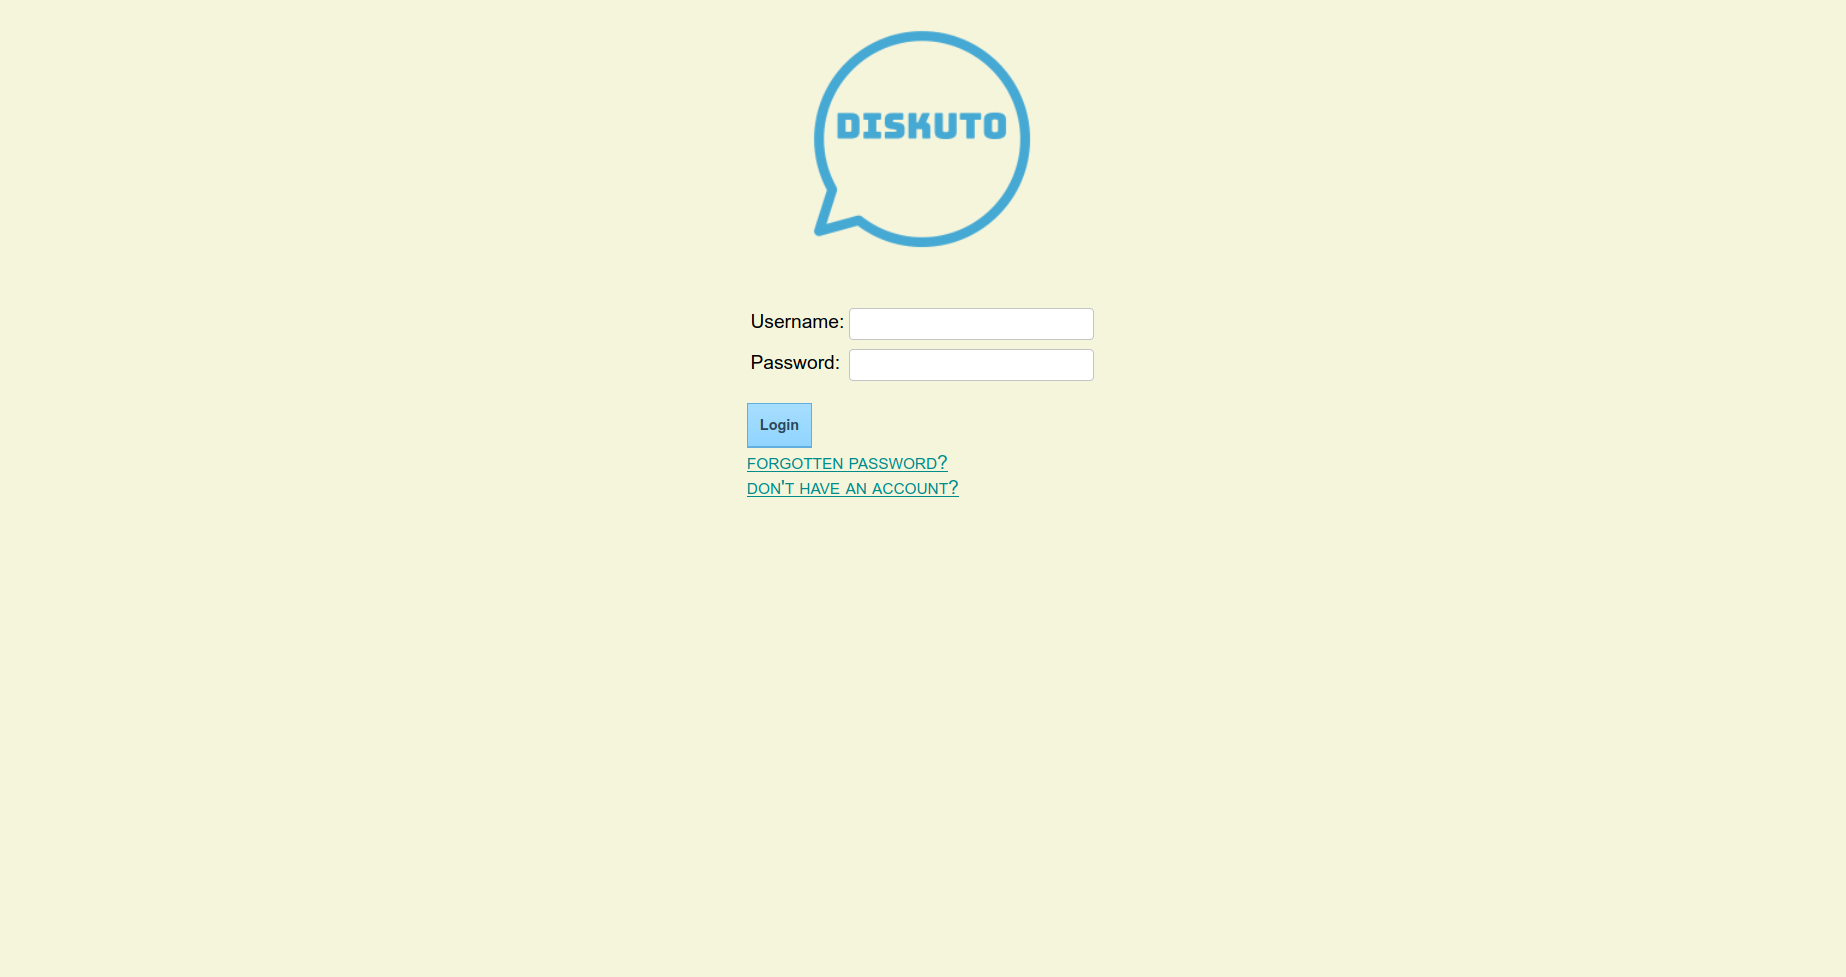
\includegraphics[width=1\textwidth]{slike/prijava.png}
    \caption{Forma za prijavu korisnika}
    \label{prijava}
\end{figure}

U zaglavlju početne stranice, odabirom na poveznicu "Login", korisnika se preusmjerava na stranicu za prijavu prikazanu na slici \ref{prijava}. Kako bi se prijavio u aplikaciju, korisnik je dužan unijeti svoje korisničko ime i lozinku. Jedino sa ispravnim korisničkim imenom i lozinkom korisnik se može prijaviti u aplikaciju, inače se korisniku javlja greška da je korisničko ime i/ili lozinka krive. Ako korisnik nema korisnički račun, pritiskom na poveznicu "Don't have an account?" preusmjerava ga se na stranicu za registraciju. Ako je korisnik zaboravio lozinku, klikom na poveznicu "Forgotten password?" otvara mu se stranica za poništavanje lozinke.

\begin{figure}[h!]
    \centering
    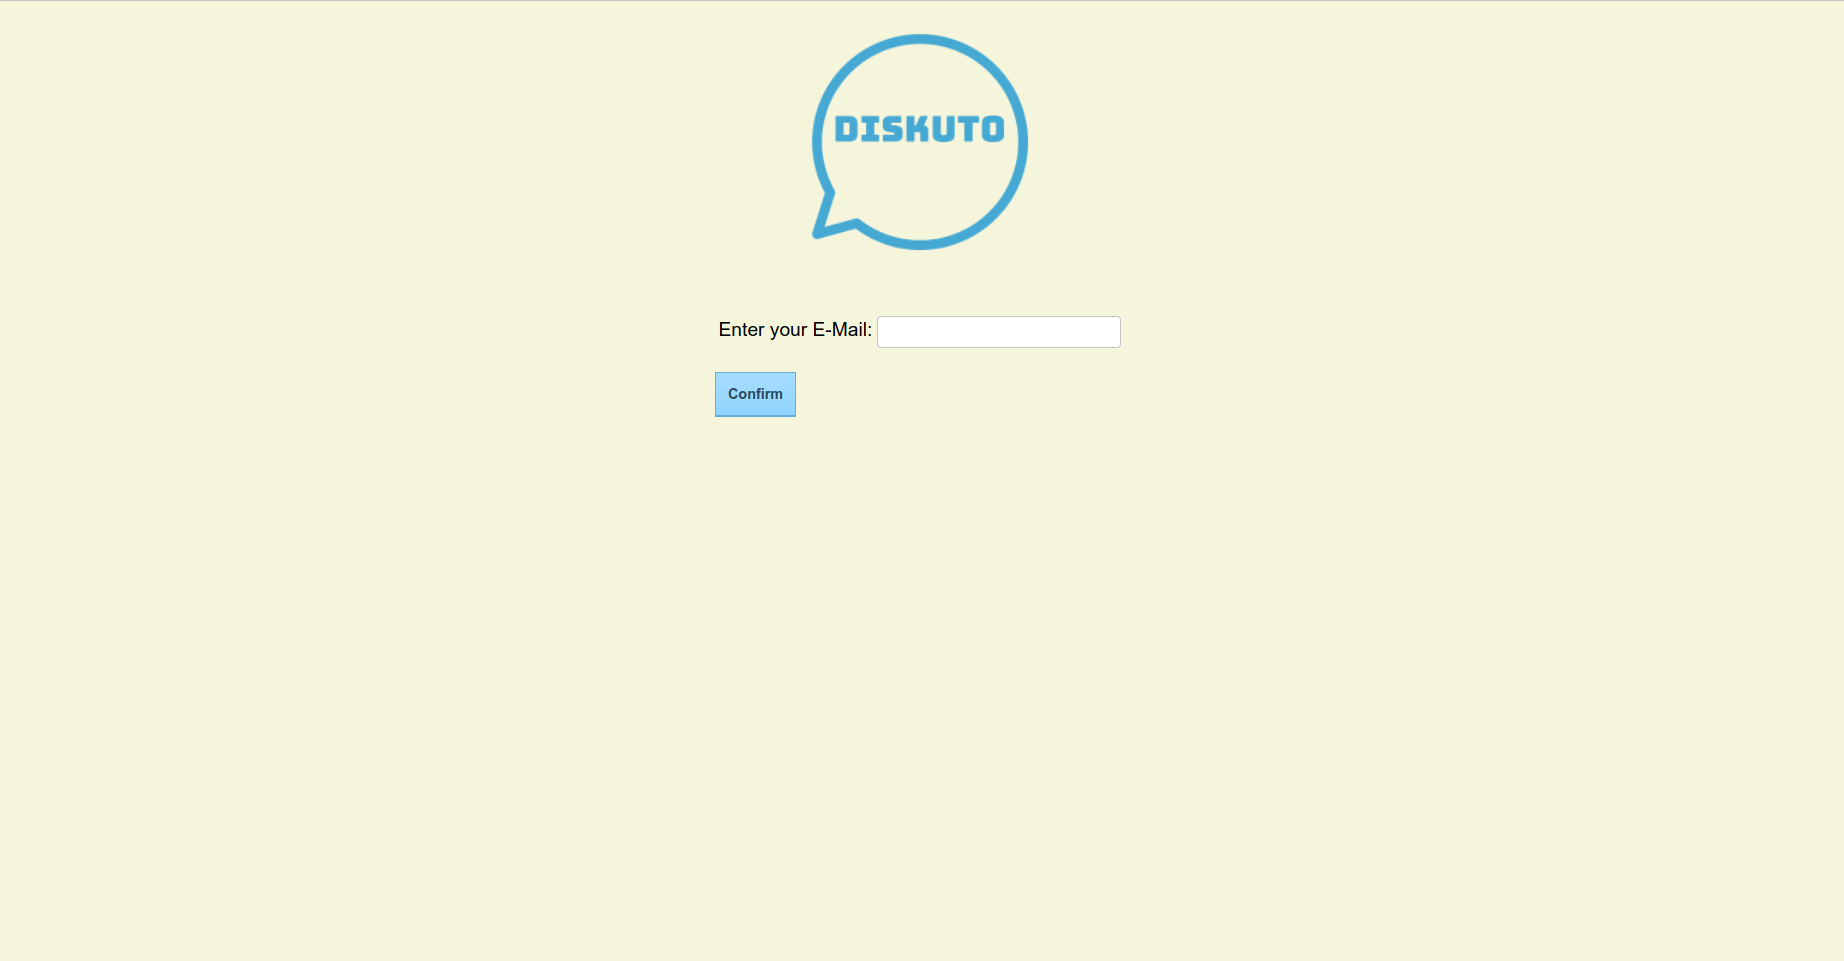
\includegraphics[width=1\textwidth]{slike/zaboravljena-lozinka.png}
    \caption{Stranica za poništavanje lozinke}
\end{figure}

Korisnik mora unijeti svoj e-mail na kojem će se poslati poveznica za kreiranje nove lozinke. Ako je e-mail nepostojeći u bazi, javit će se poruka greške. Nakon unosa pravilnog e-maila, korisniku se poništava stara lozinka i šalje mu se poruka sa uputama za kreiranje nove lozinke. U poruci će dobiti poveznicu koja ga vodi do forme za kreiranje nove lozinke. Moraju se poštivati ista pravila pri unosu lozinke kao i kod registracije (ne smije imati manje od 8 znakova i lozinka i ponovljena lozinka moraju biti jednake), u suprotnosti javit će mu se greška i korisnik neće moći obnoviti lozinku. Sve dok korisnik ne zada novu lozinku neće se moći prijaviti u aplikaciju. Obnovom lozinke korisnik se može prijaviti u aplikaciju i služiti se njome.

\section{Pronalaženje Diskuta}

Na početnoj stranici u glavnom izborniku, odabirom opcije "Pretplaćena Diskuta" (eng. "Subscribed Diskuto") korisniku se otvara stranica za pronalaženje zanimljivih foruma na koje bi se mogao pretplatiti i pratiti ih. Izgled ove stranice je prikazan na slici \ref{otkrij}.

\begin{figure}[h!]
    \centering
    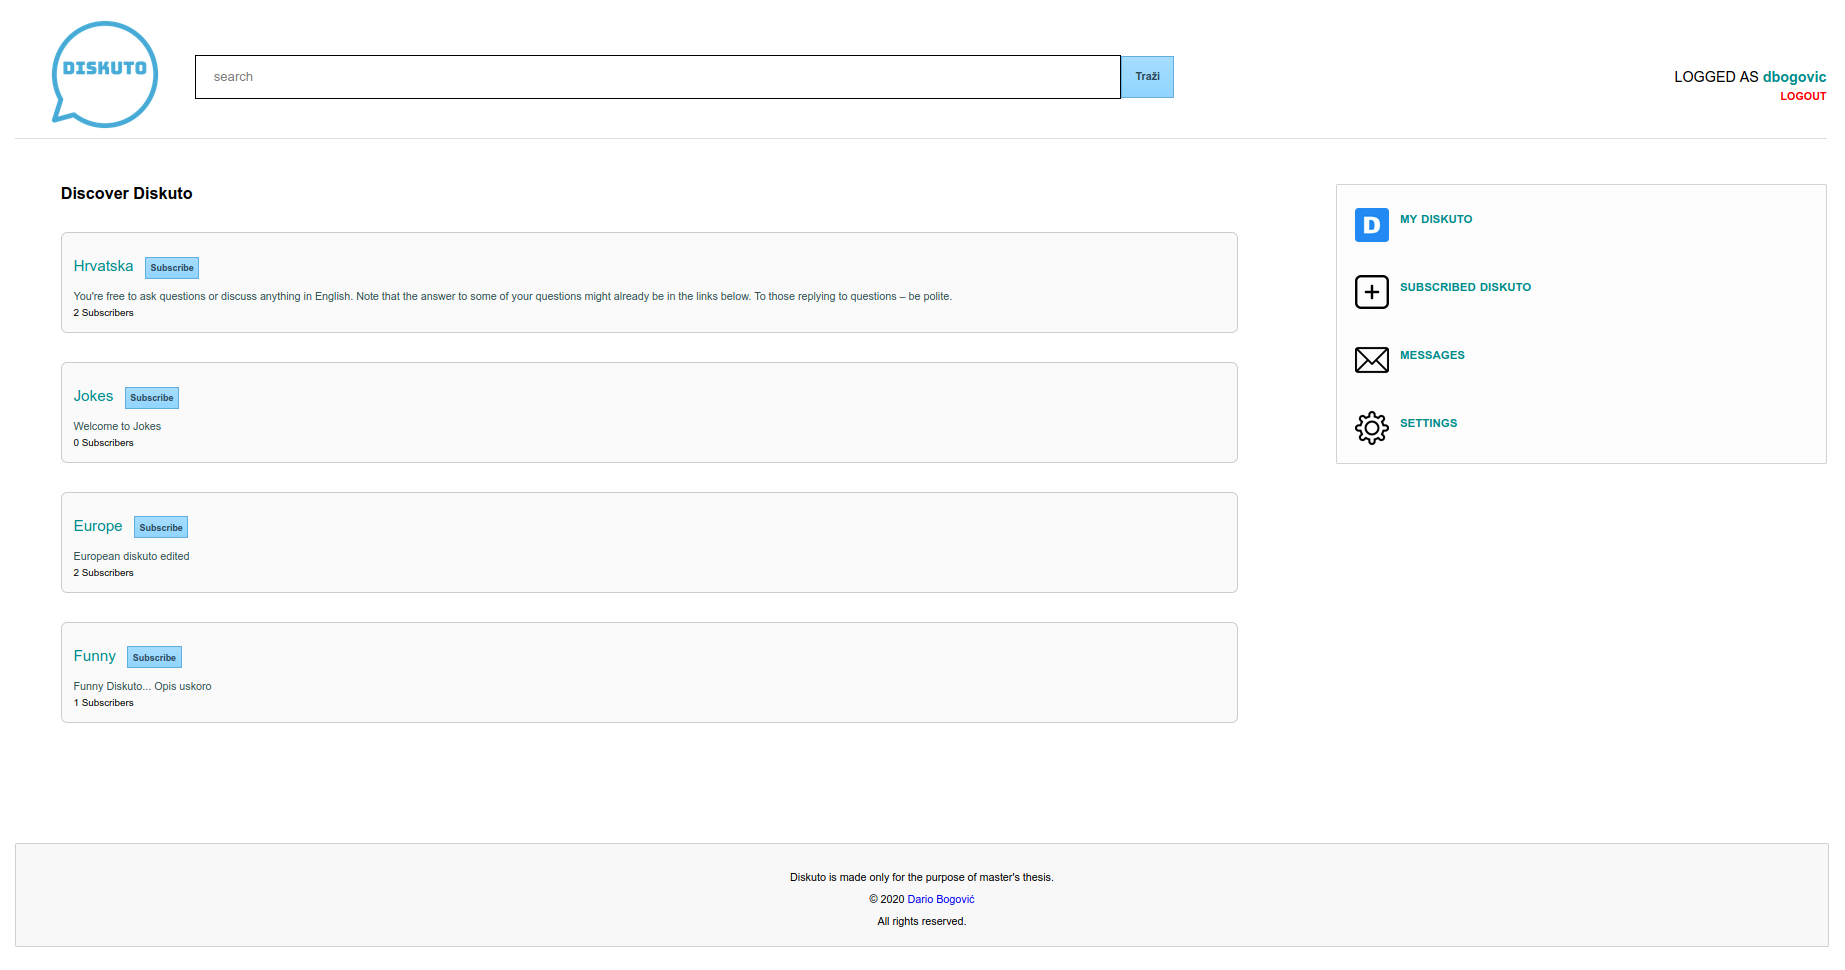
\includegraphics[width=1\textwidth]{slike/otkrij.png}
    \caption{Stranica za otkrivanje Diskuta}
    \label{otkrij}
\end{figure}

Korisniku se prikazuje popis svih foruma koji se nalaze u bazi podataka.  Za svaki pojedinačni forum je prikazan naziv, opis i broj pretplaćenih korisnika. Klikom na naziv, korisnika se preusmjerava na odabrani forum. Kraj naziva postoji jedan gumb preko kojeg je moguće pretplatiti se, odnosno ukinuti pretplatu ako već postoji pretplata na njega. Pretplatom na forum, korisnik postaje njegov član i na početnoj stranici prima najnovije objave koje su objavljene na njemu. Pretplaćeni forumi se prikazuju u glavnom izborniku odmah ispod opcije za pretragu foruma, čime korisnik može na brz i jednostavan način svojim forumima pristupiti.

\section{Kreiranje novog Diskuta}

Kako bi kreirao novi forum, korisnik se mora prebaciti na stranicu "Moja Diskuta" (eng. "My Diskuto") tako da odabere opciju u glavnom izborniku. Korisniku se tada prikazuje popis svih foruma kojih je vlasnik i na kojima je moderator. Pritiskom na gumb "Novi Diskuto" (eng. "New Diskuto"), korisniku se otvara forma za kreiranje novog foruma.

\begin{figure}[h!]
    \centering
    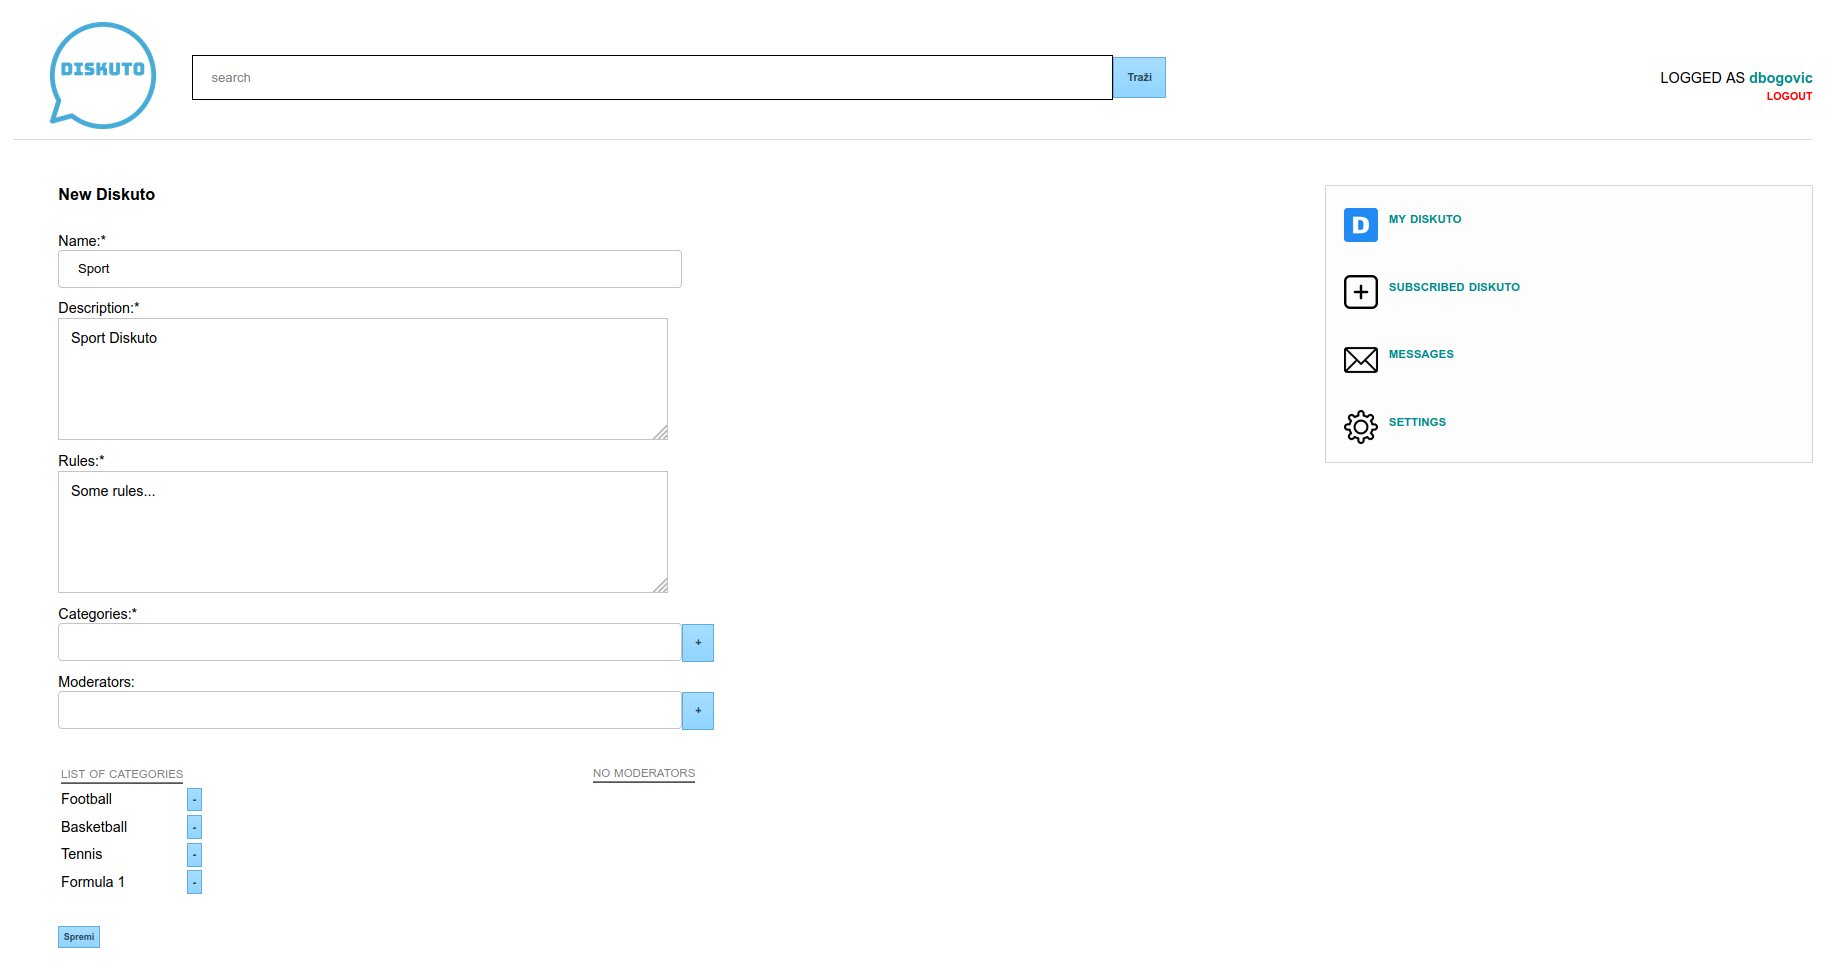
\includegraphics[width=1\textwidth]{slike/novi-forum.png}
    \caption{Forma za kreiranje novog Diskuta}
\end{figure}

Obavezno je unijeti naziv foruma, njegov opis, pravila, te barem jednu kategoriju koju će forum sadržavati. Opcionalno je moguće dodati moderatore, odnosno korisnike koji nad novokreiranim  forumom budu imali iste ovlasti kao i vlasnik. Naziv foruma je konačan i njega se nakon kreiranja ne može promijeniti, dok svi drugi atributi mogu kasnije biti modificirani. Postoji ograničenje da već ne smije postojati forum sa istim nazivom u bazi, odnosno naziv foruma se isključivo veže sa jedan i samo jedan forum. U slučaju greške korisniku će se ispisati poruka, a tek kada svi podaci budu pravilno uneseni podaci se spremaju u bazu i forum postaje kreiran.

\begin{figure}[h!]
    \centering
    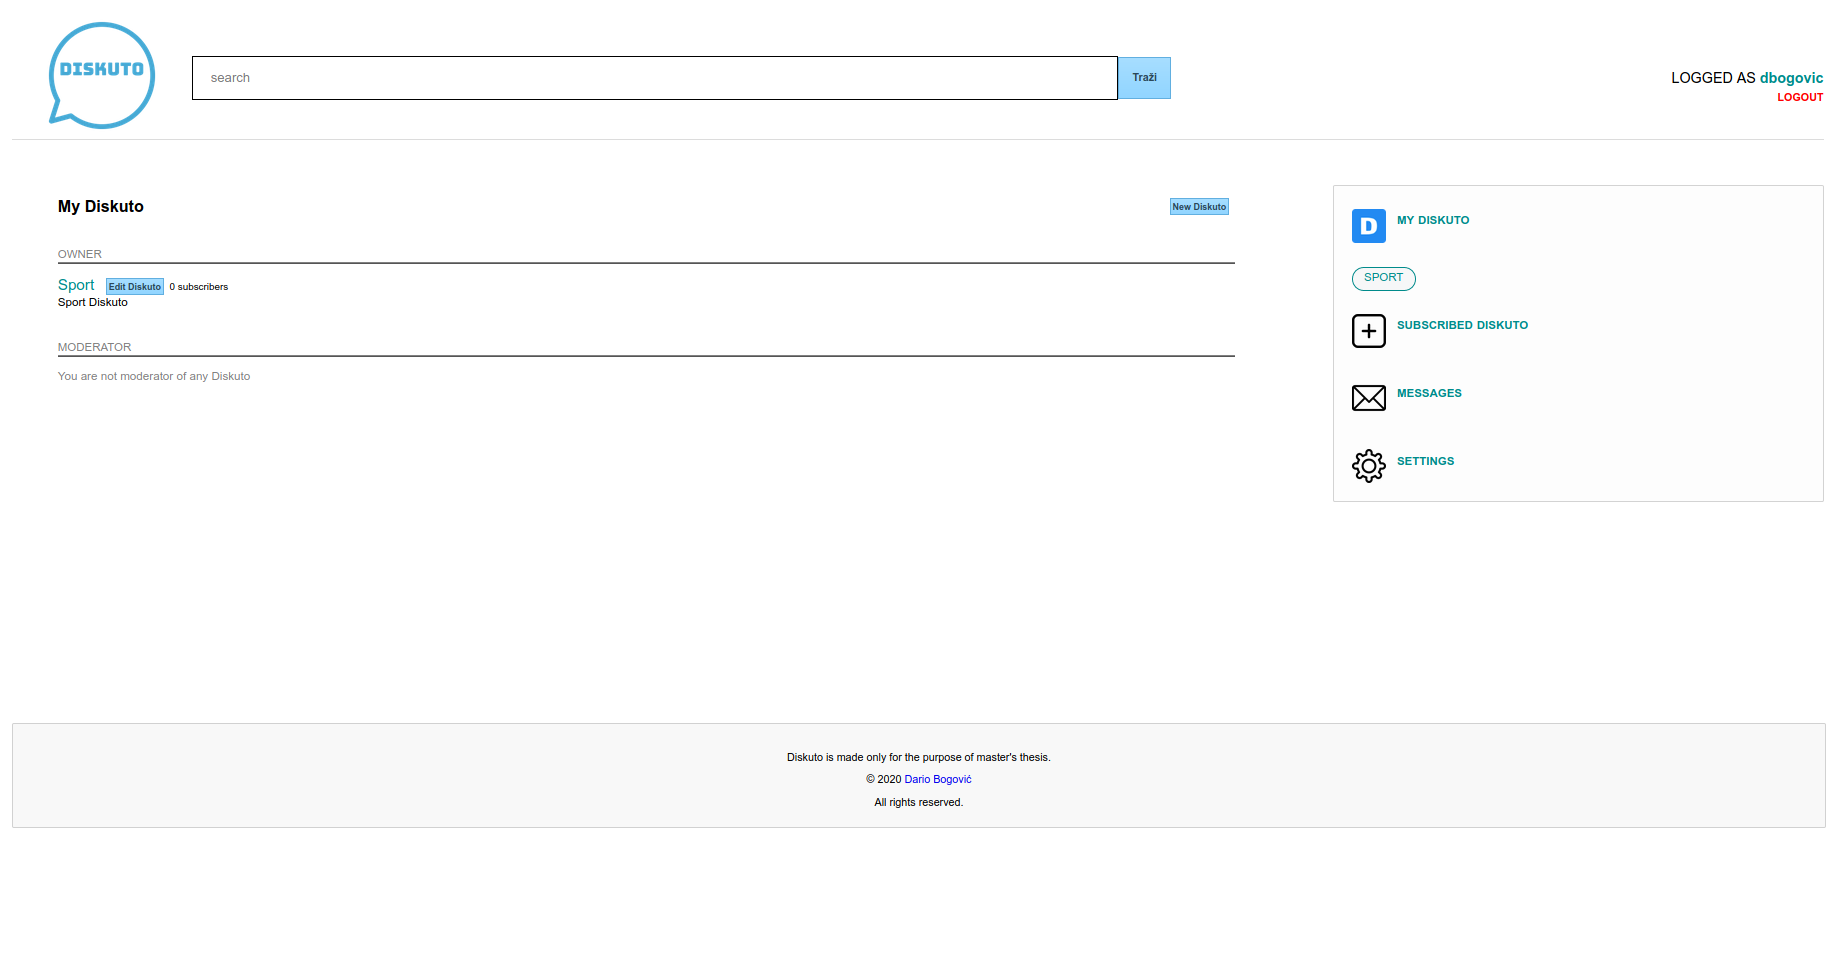
\includegraphics[width=1\textwidth]{slike/moji-forumi.png}
    \caption{Popis mojih Diskuta}
\end{figure}

Korisnika se preusmjerava na stranicu sa popisom foruma kojima je vlasnik ili moderator. Novokreirani forum se prikazuje u tablici, kao i u glavnom izborniku sa desne strane. Klikom na gumb "Uredi Diskuto" (eng. "Edit Diskuto"), korisnik može promijeniti opis i pravila foruma, brisati i dodavati kategorije, te korisnicima davati ili uklanjati ovlasti za moderatora foruma.

\section{Pregled Diskuta}

\begin{figure}[h!]
    \centering
    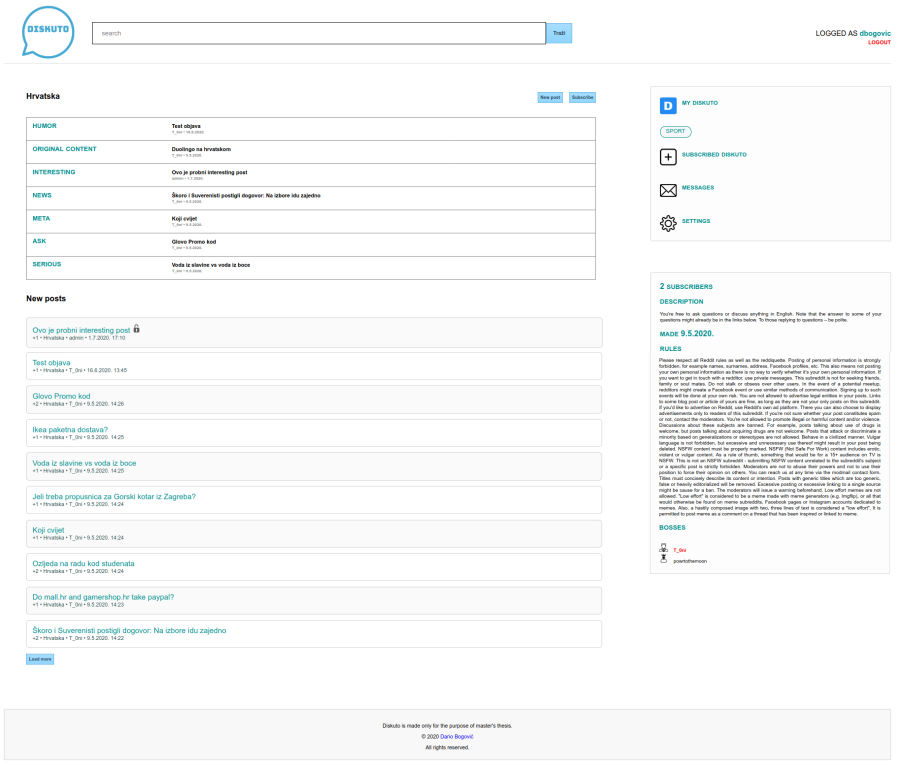
\includegraphics[width=1\textwidth]{slike/forum.png}
    \caption{Izgled stranice foruma}
    \label{forum}
\end{figure}

Na slici \ref{forum} je prikazan izgled stranice foruma za korisnika koji nije vlasnik ili moderator. Ispod glavnog izbornika aplikacije prikazan je blok sa detaljima određenog foruma: broj pretplatnika, opis, datum kreiranja, pravila foruma i poveznice na profile vlasnika i moderatora foruma.  Korisnik se može pretplatiti na forum klikom na gumb "Pretplati se" (eng. "Subscribe"), a postaviti novu objavu klikom na gumb "Nova objava" (eng. "New Post"). U glavnom dijelu aplikacije se nalazi popis svih kategorija koje forum sadrži, te sa desne strane poveznicu na najnoviju objavu na pojedinoj kategoriji. Klikom na pojedinu kategoriju otvara se popis objava sa te kategorije. Ispod elementa sa kategorijama, nalazi se popis 10 najnovijih objava na forumu i gumb za učitavanje dodatnih 10 objava. Nad svakom objavom je prikazan naslov objave odnosno poveznica nad svaku objavu, karma (odnos pluseva i minusa) koju ima, forum na kojem je objavljena, poveznica na profil vlasnika objave i datum i vrijeme kreiranja objave.

\section{Kreiranje nove objave}

\begin{figure}[h!]
    \centering
    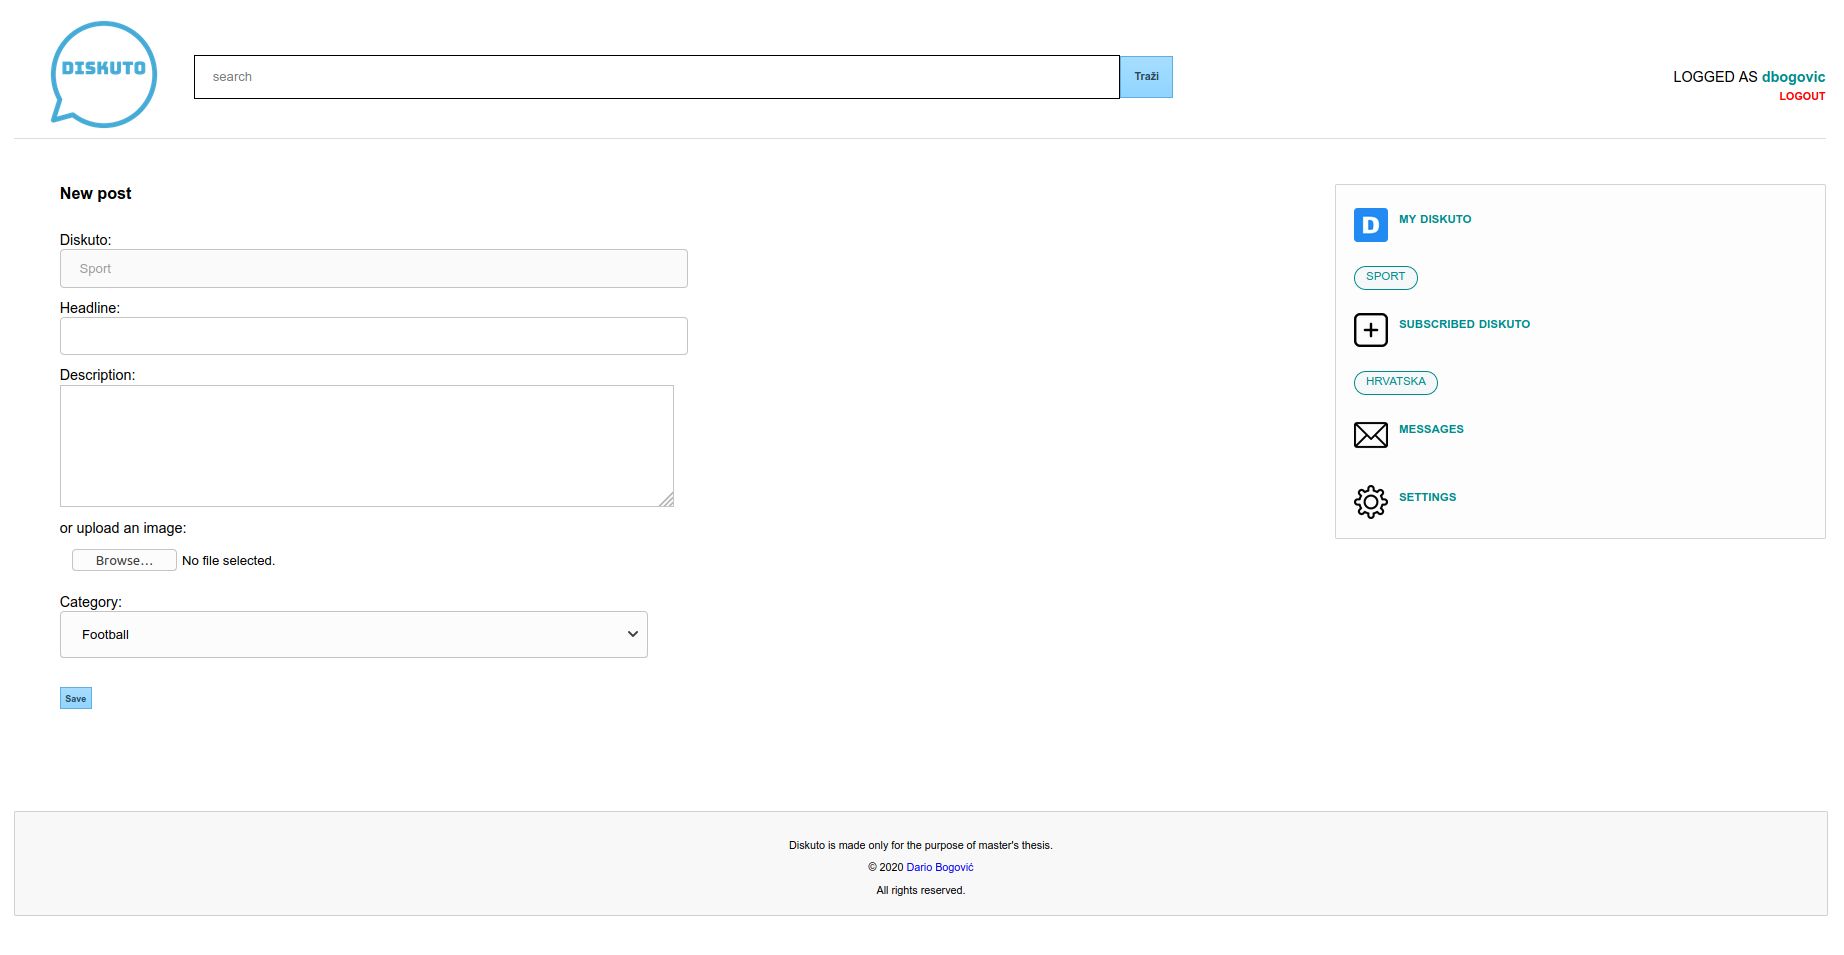
\includegraphics[width=1\textwidth]{slike/nova-objava.png}
    \caption{Forma za kreiranje nove objave}
    \label{nova-objava}
\end{figure}

Klikom na gumb za kreiranje nove objave nad pojedinim forumom, korisnika se preusmjerava na formu za kreiranje objave (slika \ref{nova-objava}). Prikazan je forum nad kojem se kreira nova objava, a korisnik mora unijeti naslov i dodatno opisati svoju objavu ili učitati sliku. Obavezno je odabrati i kategoriju na koju želi da se objava spremi. Slika koja se unosi mora biti u slikovnom formatu, a ako nije ili ako korisnik je nešto zaboravio unijeti prikazuje mu se poruka greške. Tek kada je sve u redu objava se sprema u bazu i postaje vidljiva na forumu.

\begin{figure}[h!]
    \centering
    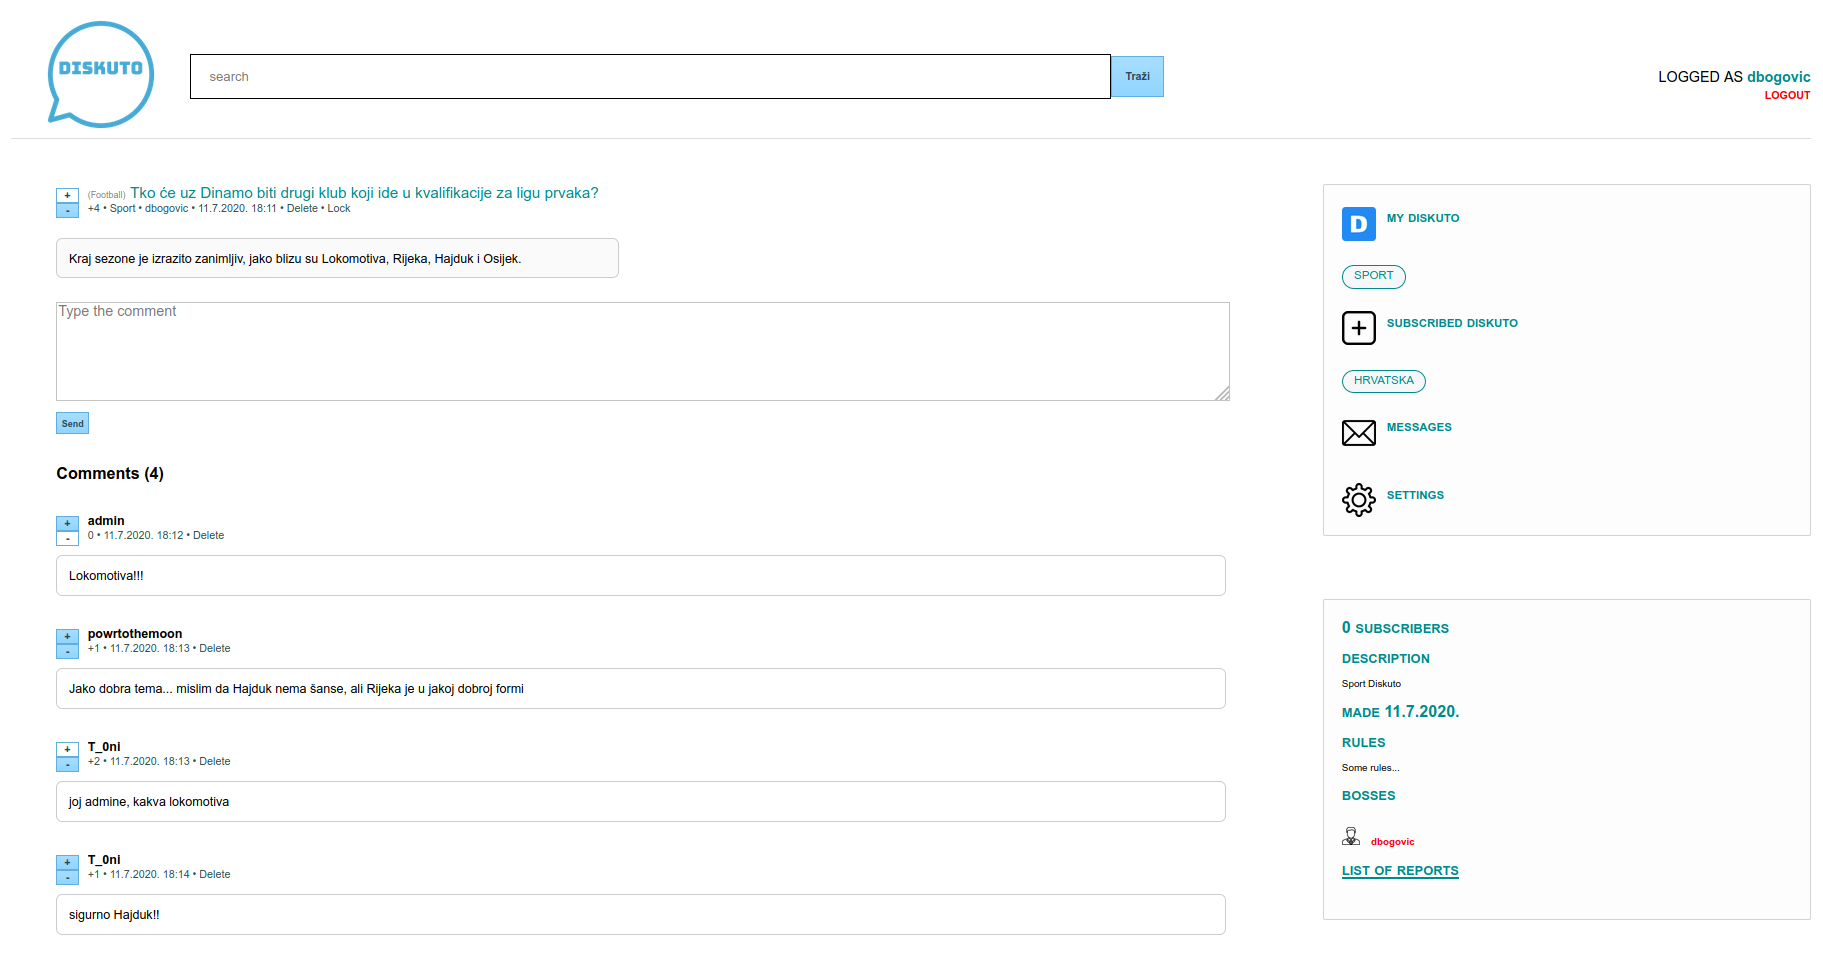
\includegraphics[width=1\textwidth]{slike/objava.png}
    \caption{Izgled objave}
    \label{objava}
\end{figure}

Izgled objave je vidljiv na slici \ref{objava}. Prikazan je naslov objave, poveznica do stranice kategorija foruma na kojem je ona objavljena, karma (odnos pluseva i minusa) koju ima, forum na kojem je objavljena, autor i vrijeme kreiranja objave. Sa lijeve strane se nalazi gumb za označavanje objave sa "+" čime se povećava karma objave i karma autora, odnosno sa "-" čime se smanjuje karma objave i karma autora. Prema zadanome autor objave automatski sam sebi zadaje "+", ali naknadno može si maknuti "+" ili si dodijeliti "-". U svakom trenutku autor objave može obrisati svoju objavu. Ako drugi korisnici foruma smatraju da objava krši pravila foruma, mogu ju prijaviti moderatorima. Ispod naslova objave slijedi tekstualni opis ili slika objave, ovisno o tome što je autor stavio kao opis. Ispod opisa se nalazi tekstualno polje za unos komentara koji se sprema u bazu pritiskom na gumb ispod njega. Zatim se nalazi element sa komentarima koji ispisuje broj ukupnih komentara i sadržaj komentara. Nad svakim komentarom se ispisuje autor objave i poveznica do njegovog profila, karma (odnos pluseva/minusa), datum i vrijeme kada je komentar postavljen, tekst komentara i gumbi sa označavanjem komentara kao "+" čime se povećava karma komentara i njegovog autora, odnosno kao "-" čime se smanjuje karma komentara i njegovog autora. Prema zadanome autor komentara automatski sam sebi zadaje "+", ali naknadno može si maknuti "+" ili si dodijeliti "-". Ispod se nalazi sami tekst komentara. U svakom trenutku autor komentara može obrisati svoj komentar. Ako drugi korisnici foruma smatraju da komentar krši pravila foruma, mogu ga prijaviti moderatorima.

\section{Ovlasti moderatora nad pojedinim Diskutom}

Kao što je već opisano u poglavlju kod kreiranja foruma, moderatori imaju naprednije ovlasti nad forumom od običnih korisnika. Imaju iste ovlasti kao i vlasnik, a oni se dodaju i brišu na stranici za uređivanje i brisanje foruma. Razlika u odnosu na vlasnika je jedino ta što je vlasnik "doživotni moderator", odnosno on ima trajne i neopozive ovlasti nad forumom. Moderatori mogu obrisati bilo koju objavu ili komentar za koji smatraju da je neprimjeren, za razliku od običnih korisnika koji jedino mogu obrisati svoju objavu/komentar. Moderatori mogu zaključati objavu i tako onemogućiti komentiranje na njoj. U svakom trenutku objava se može otključati i tako omogućiti korisnicima da nastave komentirati. Zaključane objave imaju kraj svog naslova ikonu lokota, čime ih razlikuje od drugih otključanih objava. Drugi korisnici mogu moderatorima prijaviti objave ili komentare za koje smatraju da su neprimjerene. U elementu opisa foruma, moderatori klikom na poveznicu "Popis prijava" (eng. "List of reports") mogu otvoriti stranicu sa popisom svih prijavljenih objava/komentara na njihovom forumu.

\begin{figure}[h!]
    \centering
    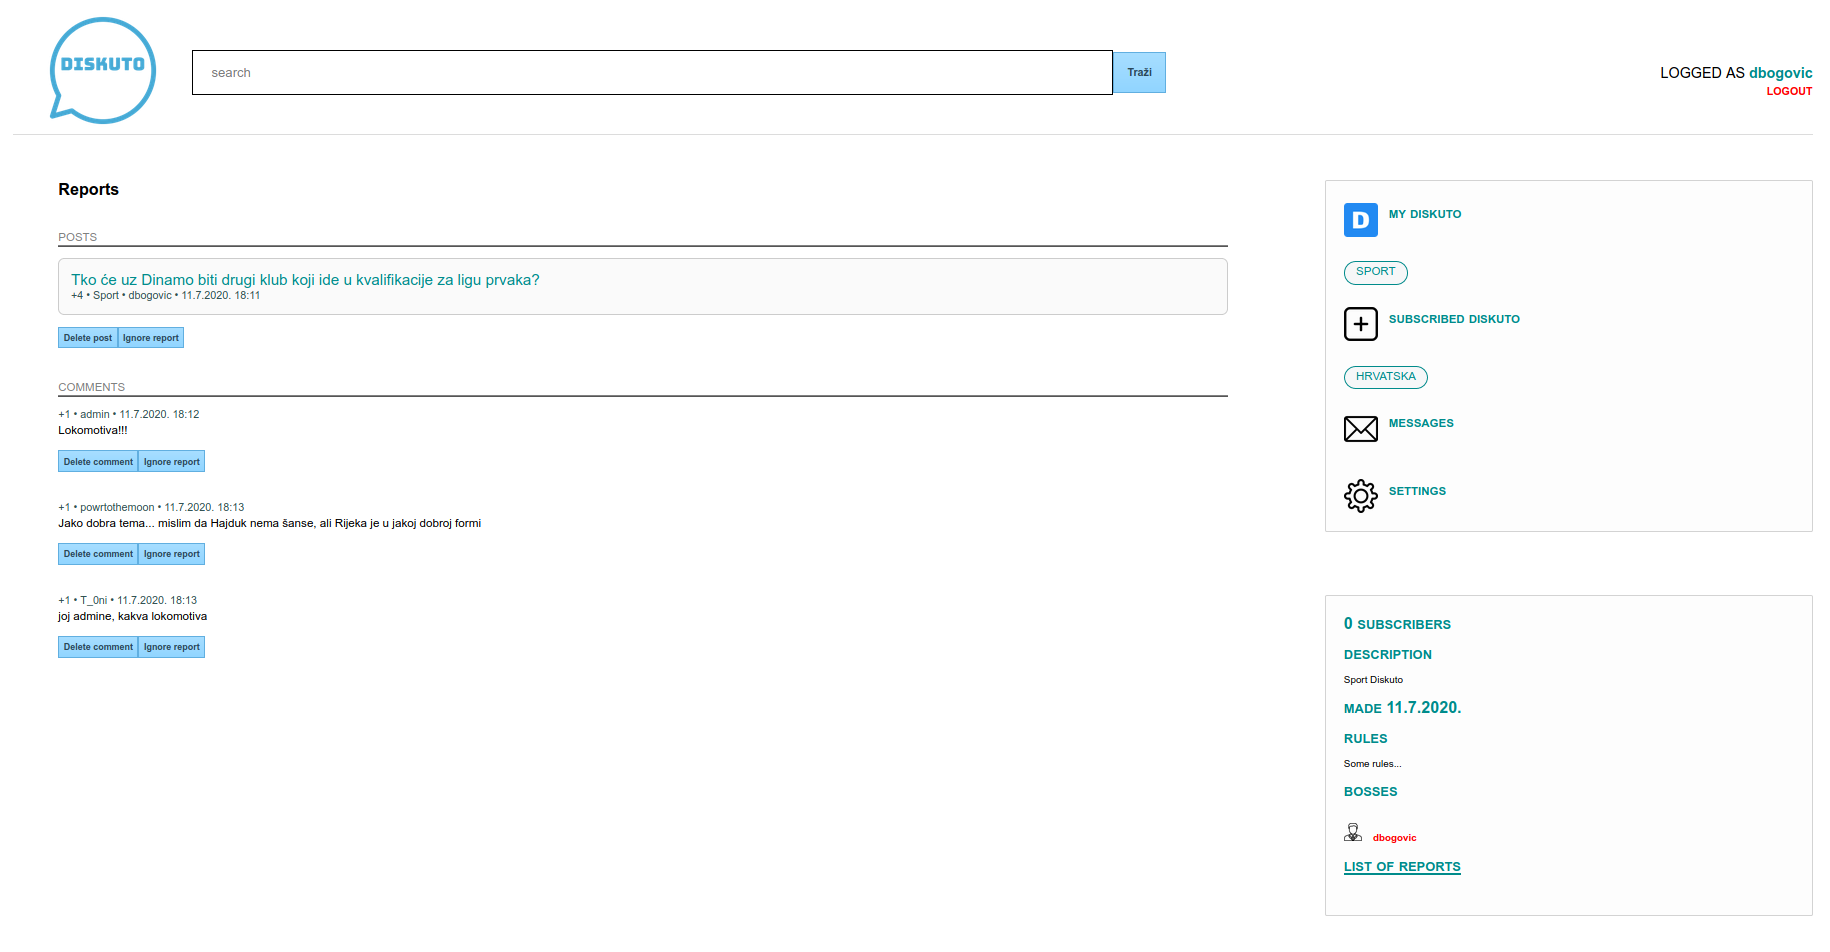
\includegraphics[width=1\textwidth]{slike/prijave.png}
    \caption{Popis prijavljenih objava/komentara}
\end{figure}

Moderatori mogu odlučiti obrisati objavu/komentar ako smatraju da krši pravila foruma ili zanemariti prijavu ako smatraju da je sve u redu.

\section{Profil korisnika}

\begin{figure}[h!]
    \centering
    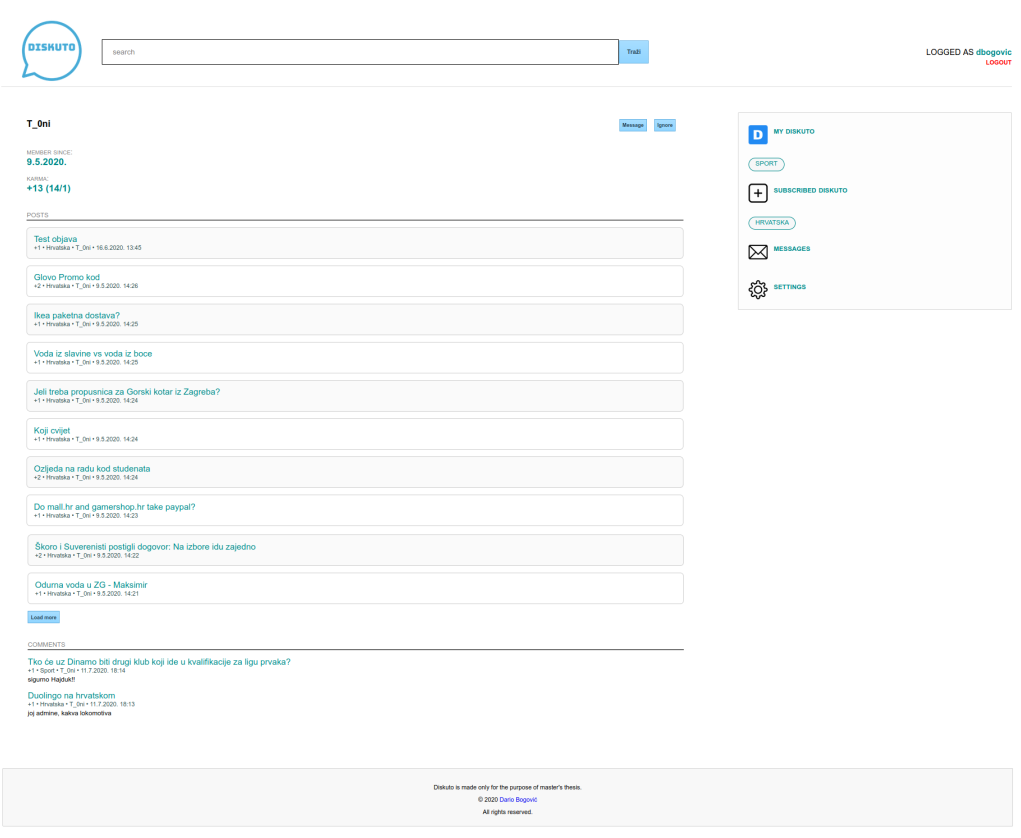
\includegraphics[width=1\textwidth]{slike/profil.png}
    \caption{Profil korisnika}
    \label{profil}
\end{figure}

Bilo gdje na stranici kada se klikne na korisničko ime pojedinog korisnika, preusmjerava se na stranicu njegovog profila kao na slici \ref{profil}. U glavnom dijelu stranice vidljivo je korisničko ime i gumbi za slanje poruke korisniku i za ignoriranje korisnika. Kada se klikne gumb za slanje poruke, korisnika se preusmjerava na stranicu sa porukama na kojoj može vidjeti prethodnu komunikaciju sa odabranim korisnikom (ako je bilo) i ima mogućnost poslati mu poruku. Naravno to je moguće ako korisnik nije drugog korisnika blokirao (ili obratno). Klikom na gumb za ignoriranje korisnik više neće vidjeti objave i komentare odabranog korisnika, kao ni primati i slati privatne poruke od njega. Deblokirati ga se može u postavkama korisničkog računa ili ako korisnik ponovno ode na njegov profil i klikne gumb za deblokiranje. Ispod naziva korisničkog imena i gumbova, mogu se vidjeti detalji o odabranom korisniku poput datuma kada je kreiran korisnički račun i ukupne karme (razlika između pluseva i minusa na svim objavama i komentarima). Ispod ovog elementa, navedene su sve objave i svi komentari pojedinog korisnika. Radi boljih performansi stranice navedeno je samo 10 njih, a klikom na gumb za učitavanje može se učitati dodatnih 10 objava/komentara. Kod objava vidljiv je naslov objave čijim odabirom se preusmjerava na samu objavu, te detalji o objavi: karma, datum kreiranja i forum na kojem je objavljen. Kod komentara vidljiv je naslov objave na kojoj je komentar objavljen i čijim odabirom se preusmjerava na samu objavu, detalji poput karme, datuma kreiranja, foruma na kojem je objavljen, te na kraju sami tekst komentara.

\section{Poruke}

Osim što korisnici mogu javno komunicirati, oni si mogu slati jedni drugima i privatne poruke. Korisnik inicira razgovor sa drugim korisnikom odabirom gumba za slanje poruka na njegovom privatnom profilu. Tada se korisnika preusmjerava na stranicu sa porukama kojoj se može pristupiti i sa glavnog izbornika odabirom opcije "Poruke" (eng. "Messages"). 

\begin{figure}[h!]
    \centering
    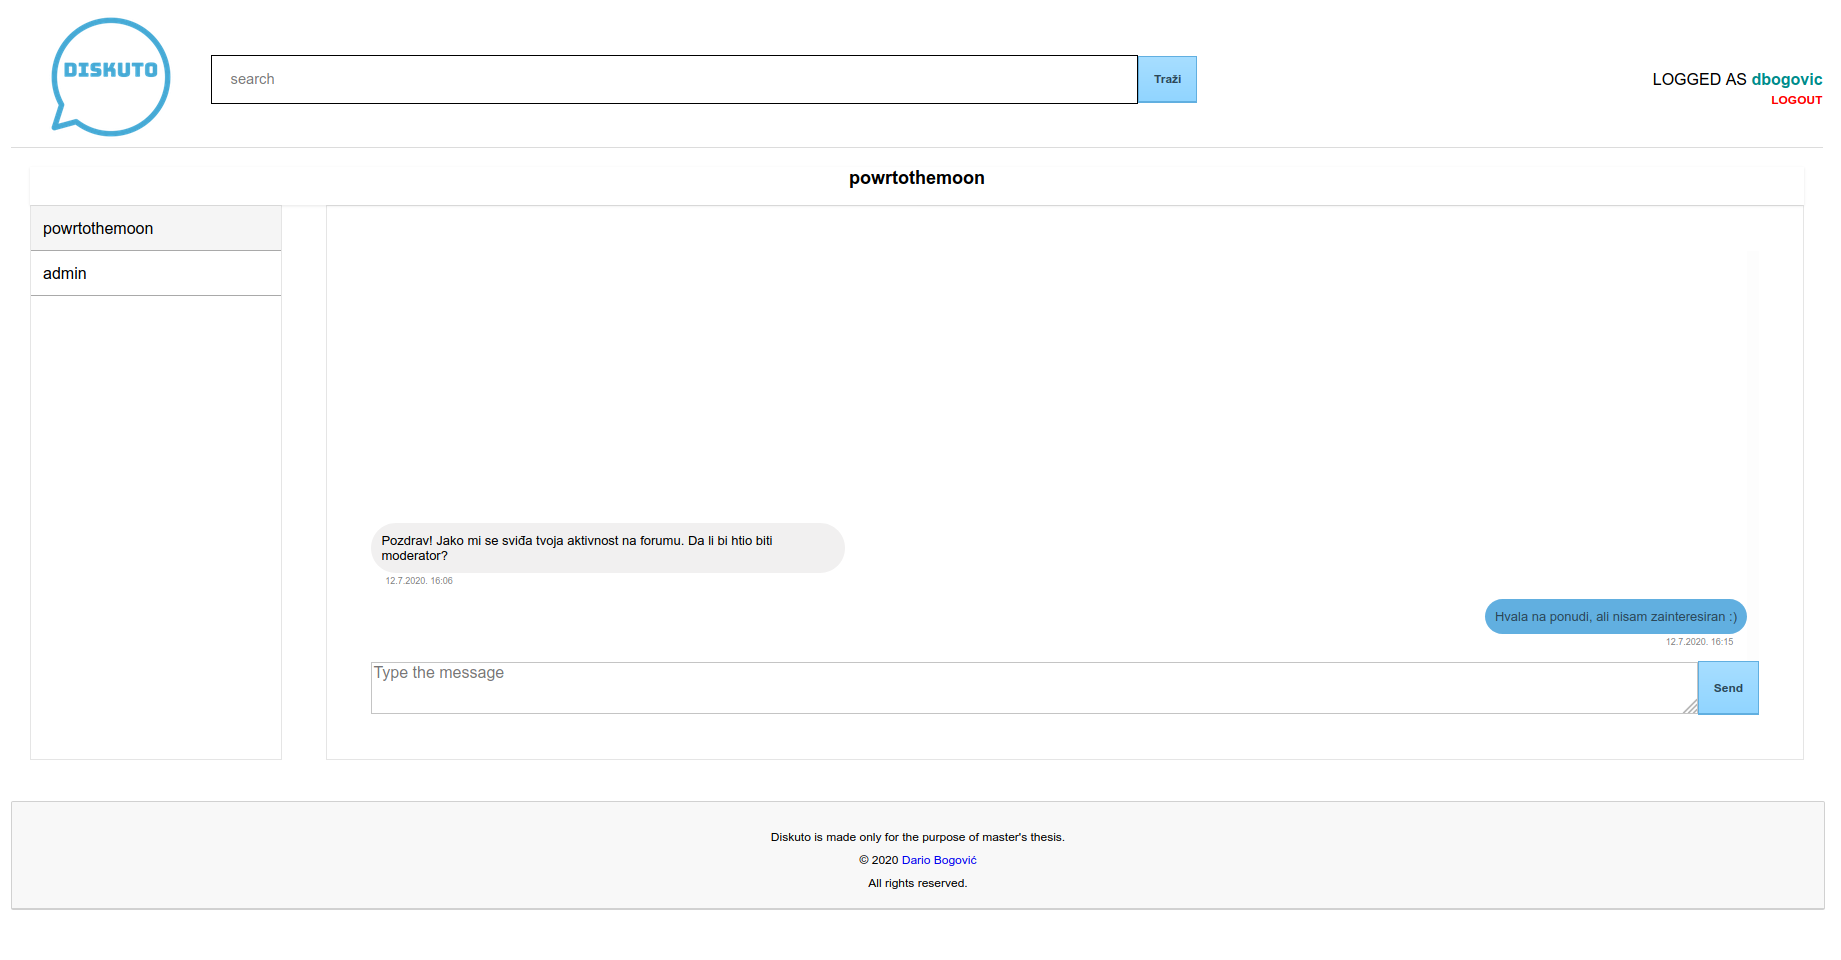
\includegraphics[width=1\textwidth]{slike/poruke.png}
    \caption{Poruke}
    \label{poruke}
\end{figure}

Prikaz stranice za slanje privatnih poruka je vidljiv na slici \ref{poruke}. Između zaglavlja i podnožja stranice nalazi se glavni dio stranice koji se sastoji od: korisničkog imena korisnika sa kojim je trenutno aktivna komunikacija i poveznica na njegov profil, s lijeve strane popis svih korisnika sa kojima je korisnik komunicirao u prošlosti i poveznica na njihovu stranicu komunikacije, te u glavnom dijelu se nalaze same poruke koje su si korisnici međusobno razmijenili. Poruke koje je korisnik primio su poravnate sa lijeve strane i imaju crnu boju teksta na sivoj pozadini. Poruke koje je korisnik poslao su poravnate sa desne strane i imaju tamnoplavu boju teksta na plavoj pozadini. Ispod svake poruke nalazi se točan datum i vrijeme kada je poruka poslana ili primljena. Ispod elementa sa porukama nalazi se tekstualni element za slanje poruke. Poruku je jedino moguće poslati ako se korisnici ne ignoriraju, odnosno ako jedan nije stavio drugoga na listu ignoriranja. Kada pošiljatelj pošalje poruku, primatelja se obaviještava na način da u glavnom izborniku aplikacije mu se prikaže da ima nepročitanu poruku i ispod mu se prikaže na poveznicu razgovora sa korisnikom od kojeg je primio poruku. Sve dok primatelj poruku ne pročita, ta će mu obavijest biti prikazana u glavnom izborniku.

\section{Pretraga}

Tijekom većine vremena služenja sa aplikacijom se u zaglavlju nalazi traka za pretragu foruma. Registrirani korisnici mogu pretražiti po ključnoj riječi sve forume, korisnike i objave na forumima. Ako ključna riječ je sadržana u nazivu foruma, korisničkom imenu korisnika ili naslovu objave na nekom forumu ona će se prikazati kao rezultat pretrage.

\begin{figure}[h!]
    \centering
    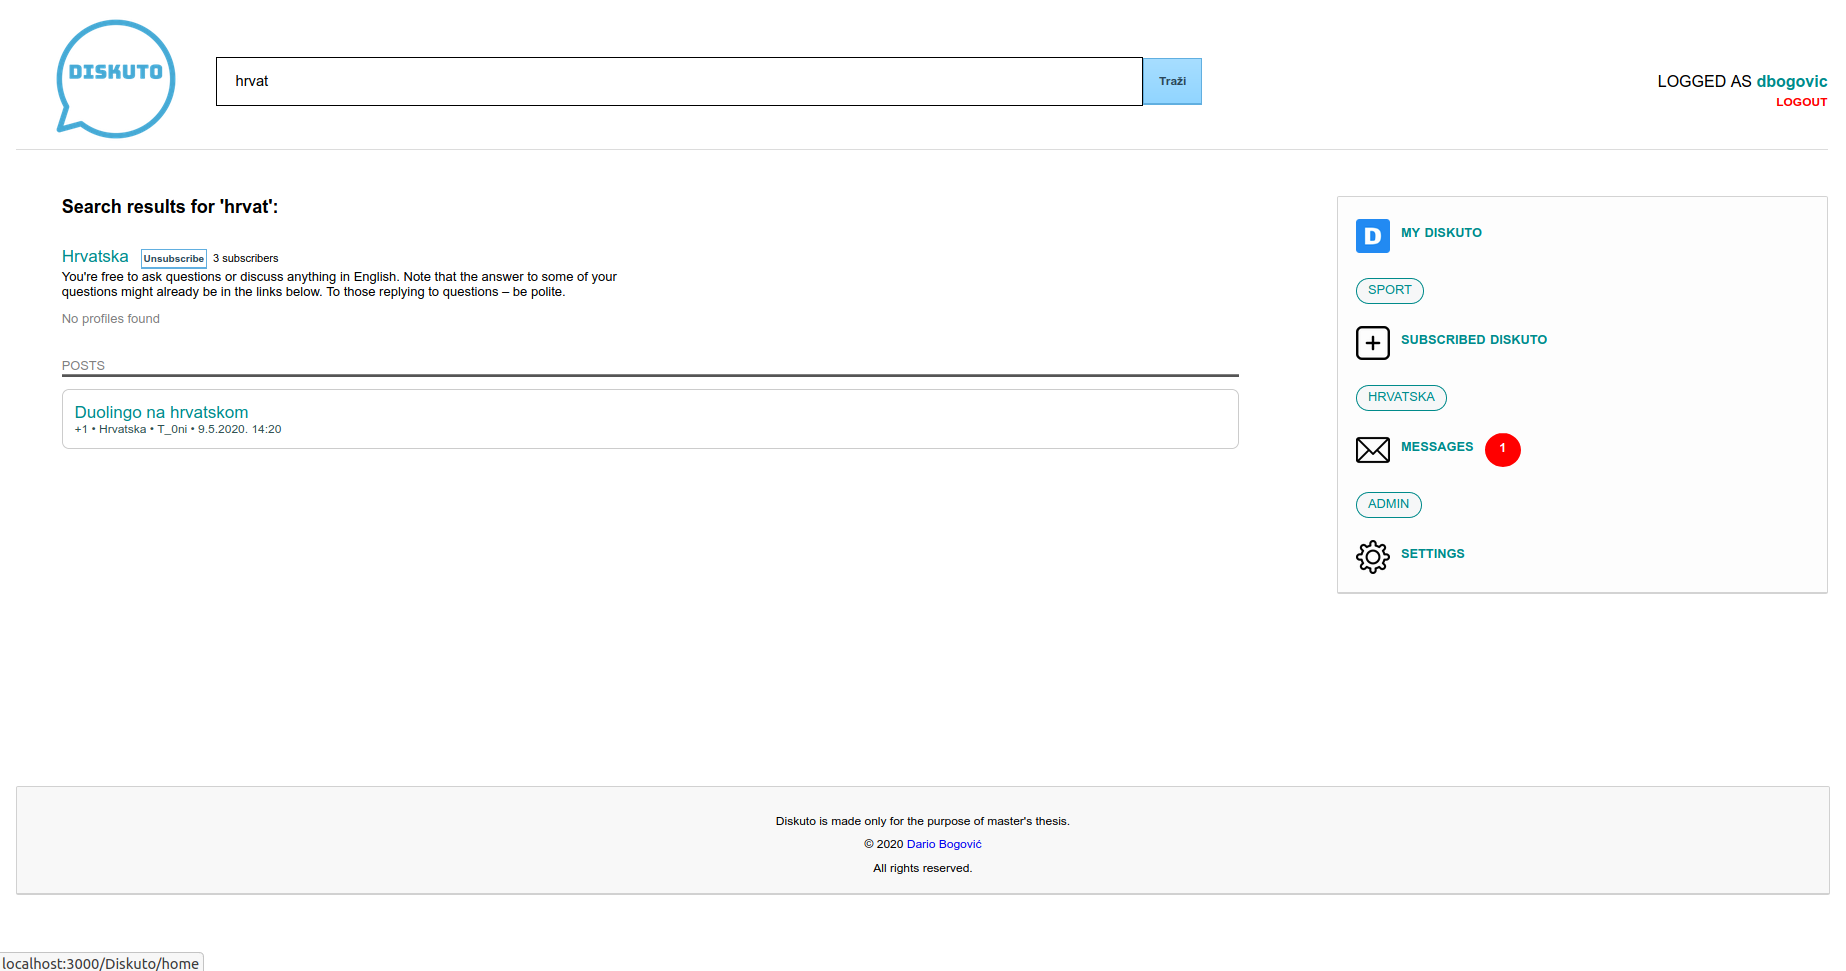
\includegraphics[width=1\textwidth]{slike/pretraga.png}
    \caption{Izgled stranice za pretragu}
    \label{pretraga}
\end{figure}

Na slici \ref{pretraga} je prikazan primjer izgleda stranice za pretragu ako je unesena ključna riječ "hrvat". Vidljivo je kako je aplikacija vratila kao rezultat pretrage jedan forum pod nazivom "Hrvatska", niti jedan profil sa korisničkim imenom koji sadrži tu ključnu riječ, te jednu objavu koja u sebi sadrži ključnu riječ "hrvat". Ako aplikacija vrati forum kao rezultat pretrage, ona će ispisati naziv foruma koja je poveznica na stranicu foruma, gumb za pretplatu/poništenje pretplate i detalje o forumu poput broja pretplaćenih korisnika i opis. Ako aplikacija vrati korisnika kao rezultat pretrage, ona će ispisati korisničko ime koje je ujedno i poveznica na profil, te gumb čijim klikom se preusmjerava na slanje privatne poruke. Ako aplikacija vrati objavu kao rezultat pretrage, ispisat će se puni naslov objave koja je i poveznica na samu objavu, te detalji o objavi poput karme (razlika pluseva/minusa), poveznica na forum gdje je objava objavljena, poveznica na profil autora objave i datum i vrijeme kada je objava objavljena. Ako aplikacija ne vrati niti jedan forum, korisnika ili objavu ispisat će se obavijest o neuspjehu.

\section{Postavke}

\begin{figure}[h!]
    \centering
    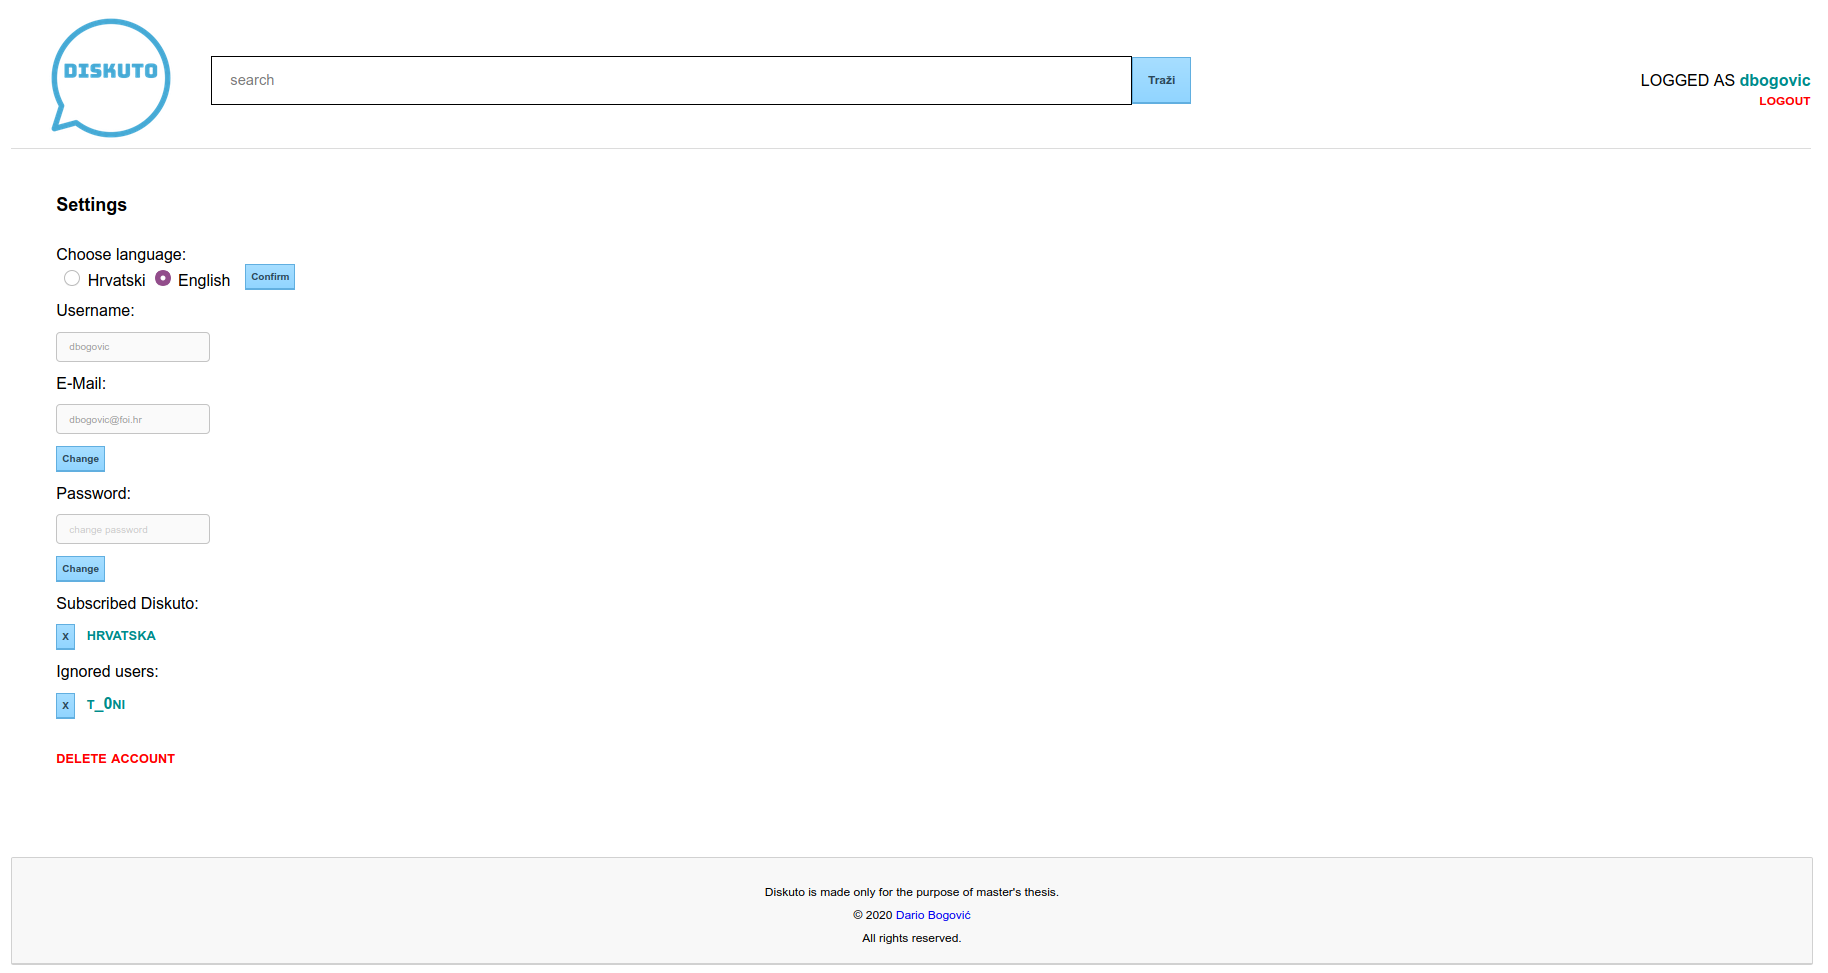
\includegraphics[width=1\textwidth]{slike/postavke.png}
    \caption{Korisničke postavke}
\end{figure}

Korisničkim postavkama se može pristupiti odabirom opcije "Postavke" (eng. "Settings") u glavnom izborniku aplikacije. Korisnik može promijeniti jezik aplikacije, a na raspolaganju su mu dva jezika: engleski i hrvatski. Klikom na gumb za promjenu spremaju se postavke i u bazi, pa kada se korisnik ponovno prijavi prikazati će mu se željeni jezik kojeg je promijenio u postavkama. Korisničko ime je nepromijenjivo, te ga se nakon registracije ne može mijenjati. Korisnik može promijeniti e-mail tako da nakon što klikne gumb za promjenu umjesto sadašnjeg unese novi e-mail. Ako unese krivi format, aplikacija mu neće dozvoliti promijenu i ispisat će se greška. Korisnik može promijeniti i svoju lozinku tako da nakon što klikne gumb za promjenu unese novu lozinku. I dalje stoji pravilo da lozinka ne smije biti preslaba, odnosno ne smije imati manje od osam znakova. Ako je lozinka preslaba, aplikacija mu neće dozvoliti promijenu lozinke i ispisat će se greška. Korisnik također može vidjeti na koje forume je trenutno pretplaćen, te klikom na gumb "X" koji stoji pokraj poveznice na forum može ukloniti pretplatu. Korisnik može vidjeti i koje je korisnike blokirao, te klikom na gumb "X" koji stoji pokraj poveznice na njegov profil može ga deblokirati. Klikom na opciju "Obriši račun" (eng. "Delete account") korisnik može trajno obrisati svoj račun. Za potvrdu je potrebno unijeti trenutnu lozinku. Ako je lozinka pogrešna ispisat će se greška, a ako unese dobru lozinku i potvrdi je račun se trajno briše i prikazuje mu se poruka kao na slici:

\begin{figure}[h!]
    \centering
    
\includegraphics[width=1\textwidth]{slike/deaktivacija.png}
    \caption{Poruka o deaktiviranom računu}
\end{figure}

\chapter{Zaključak}

\printbibliography[title=Popis literature]
\addcontentsline{toc}{chapter}{Popis literature}

\listoffigures
\addcontentsline{toc}{chapter}{Popis slika} 

\listoftables
\addcontentsline{toc}{chapter}{Popis tablica}

\end{document}
